\chapter{Results and methods}
In the present chapter, the original methodologies and results of the experimental process are displayed; they were collected and developed during the thesis research with the aim of devising MD simulations that are of relevant scientific interest. 
%Nel presente capitolo sono illustrate le metodologie ed i risultati del lavoro sperimentale svolto in maniera originale nel corso della tesi per sviluppare delle particolari simulazioni di dinamica molecolare di alcuni sistemi di interesse scientifico.

The systems that were mainly analyzed \textit{in silico} were powder solutions of proteins and water (i.e. solutions that are barely hydrated). The study of systems with a low hydration, is not only scientifically relevant, but it turns out to be very interesting from a perspective of the possible applications, for example for fields of applications that concern the study and projection of pharmaceuticals where the main active substance are proteins.\footnote{With the significant advancements in biologics and biopharmaceutical over the years, peptides and proteins have emerged with a host of new applications in the diagnostic as well as the therapeutic sector. As for the current calculations, the market for peptide and protein drugs is estimated around 10\% of the entire pharmaceutical market and will make up an even larger proportion of the market in the future. Since early 1980s, a total 239 therapeutic proteins and peptides are approved for clinical use by US-FDA (United States -- Food and Drug Administration [\url{10.1371/journal.pone.0181748}]}
%In particolare, i sistemi prevalentemente analizzati in silico sono soluzioni in polvere (ovvero poco idratate) di proteine e acqua. Lo studio di questo tipo di sistemi con una bassa percentuale di idratazione, oltre che da un punto di vista puramente scientifico, risulta molto ineteressante anche da un punto di vista applicativo per quanto riguarda, per esempio, campi di ricerca che concernono lo studio e la progettazione di farmaci in cui il principio attivo è costituito da proteine
 
For this reason, systems of proteins in powder are widely studied experimentally, principally through neutron spectroscopy. 
%Per questo, sistemi di proteine in polveri sono molto studiati sperimentalmente e, in particolare, questo viene fatto di solito attraverso la spettroscopia neutronica.
This technique, which is sensitive to the dynamics and the structure of condensed matter on the atomic scale, gives precise information about the mean atomic fluctuations and the dynamics in proteins, enhancing an average view of all atomic contributions.
However, due to the high complexity of these systems, usually their internal dynamics is too complicated for a quantitative interpretation at an atomistic detail starting from the average information obtained from neutron scattering.

In this context, computer simulations, and in particular Molecular Dynamics (MD) simulations, enable to gain a wider insight into the dynamics of proteins that are not provided from neutron scattering and from any real experiments, in general. 
Simulated trajectories can be analyzed in detail and information not accessible from experiments can be extracted from computer simulations.\footnote{For some interesting applications, on to the interpretation of neutron scattering, see the Kneller's lecture: ``\textit{Quasielastic Neutron Scattering}'' \cite{ref:QNS_Keller}.}

The objective of this thesis is precisely that of performing apo and holo simulations of a specific protein in powder environments that will enhance to collect valuable information about the interactions that contribute to the formation of the protein-ligand complex. In particular this protein and the ligand are:
%L'obbiettivo di questa tesi è infatti proprio quello di realizzare delle simulazioni delle forme apo e holo di una particolare proteina in ambienti polvesi che potranno permettere di ricavare preziose informazioni sull'interazioni che contribuiscono alla formazione del protein-ligand complex. Nello specifico, the protein and the ligand simulated are:
\begin{center}
\begin{minipage}{0.65\textwidth}
\begin{itemize}
\item[\textbf{Protein:}] Maltose-Binding Protein (MBP), also known as Maltosedextrin-Binding Protein
\vspace{-0.2cm}
\item[\textbf{Ligand:}] Maltose (Malt)
\end{itemize}
\end{minipage}
\end{center}
The MBP is a well studied model protein that plays an important role in the metabolism of Escherichia coli, e.g., in the energy-dependent translocation of maltose and maltodextrins through the cytoplasmic membrane \cite{paciaroni2008fingerprints}.\\

%sebbene esistano diversi software per realizzare delle simulazioni di MD per studiare biomolecole, nel caso di sistemi scarsamente idratati   delle proteine proteine simulazioni di proteine in ambienti scarsamente idratati non sono abbasta

%Pertanto, nella prima sezione è descritta la realizzazione delle varie simulazioni realizzate nel corso della tesi. Nella seconda e nella terza sezione, invece, sono riportate alcune misure ottenute dell'analisi delle traiettorie simulate per studiare ...
In the first section, the implementation of the several simulations performed during the thesis research are described. 
In the second and third section the measurements obtained from the simulated trajectory analysis are reported...

\section{Simulations}
\subsection{Problems with powders}
In most part of the cases, the studied systems in biology are abundantly hydrated. For this reason, programs like NAMD, that allow to create accurate and efficient simulations of biological systems rapidly enough, are developed considering principally very diluted systems. In the case of the simulations of proteins in powders, the performing of simulations is notably much more difficult. In particular, due to the scarceness of water molecules, the building of the initial state can become quite cumbersome and difficult.
%Nella maggior parte dei casi, i sistemi studiati in ambito biologico sono abbondantemente idratati. Per questo motivo programmi come NAMD \cite{ref:NAMD}, che permettono di creare abbastanza rapidamente delle simulazioni di sistemi biologici il più possibile accurate ed efficienti, sono sviluppati considerando principalemente sistemi molto diluti. Nel caso delle simulazioni di proteine in polveri, tuttavia, la realizzazione delle simulazioni si complica notevolemente. In particolare, a causa della scarsità di molecole d'acqua, la costruzione dello stato iniziale può risultare abbastanza difficoltosa.

When studying the dynamics of proteins in very diluted systems, frequently it is sufficient to simulate a single protein in a water box that is big enough to avoid the auto-interaction of the protein with itself, caused by the periodic boundary conditions. In these systems, it is easy to construct the box with a setting where the water molecules that are randomly arranged inside the box, surround completely the protein and fulfill the box entirely in a quite uniform distribution.
%Per studiare la dinamica delle proteine in sistemi molto diluiti, di solito è sufficiente simulare una sola proteina in una box d'acqua abbastanza grande da evitare l'autointerazione della proteina con se stessa a causa delle condizioni di periodicità al contorno. In questi sistemi, è facile costruire queste box in modo tale che le molecole d'acqua, disposte casualemente all'interno della box, circondino totalmente la proteina e riempiono la completamente la box in modo abbastanza uniforme. 

\begin{figure}[H]
\centering
\begin{minipage}[t]{0.7\textwidth}
	\centering
    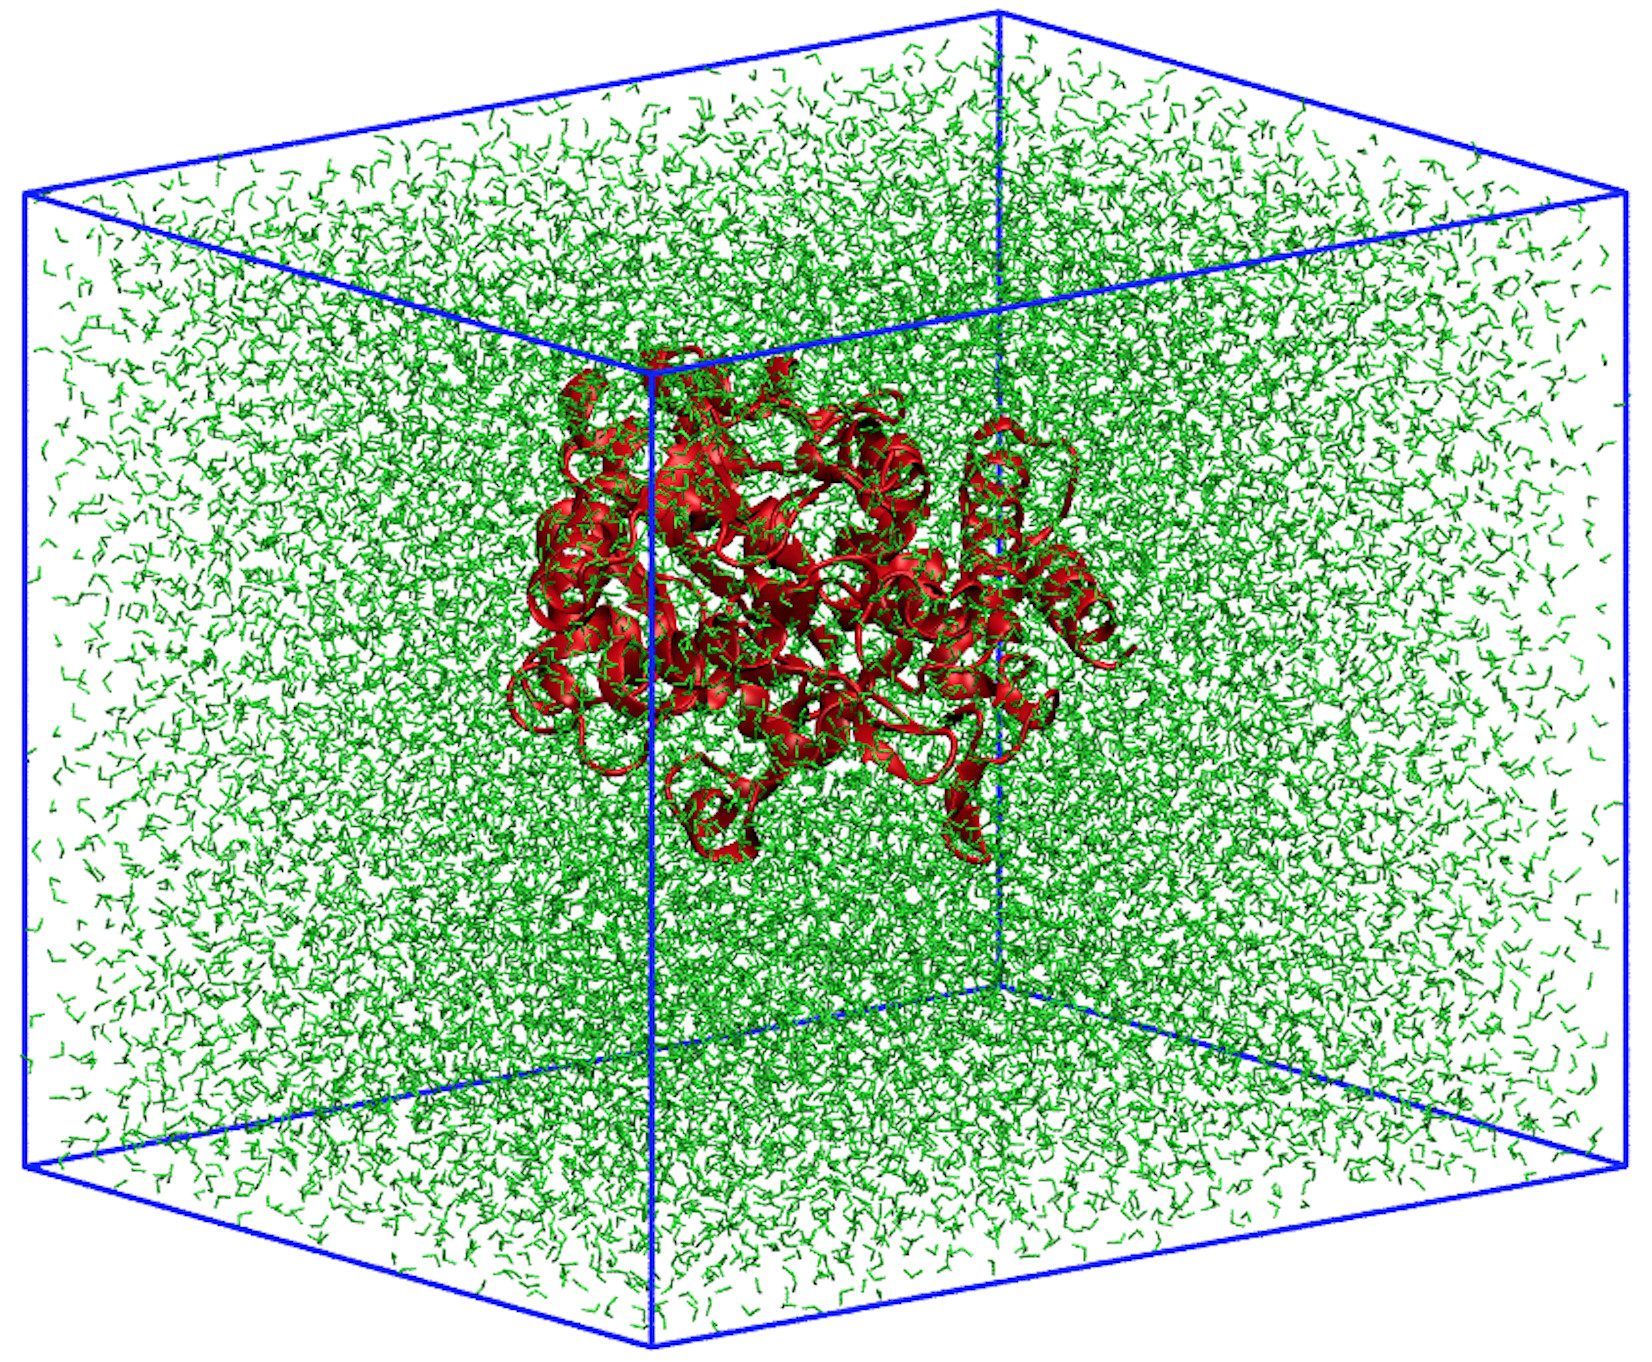
\includegraphics[width=0.70\textwidth]{dil-1omp.jpg}
    
    \footnotesize{\caption{Example of a MBP in a highly hydrated cubic box of $80 \times 80 \times 80$ $\AA^3$. \textit{Picture realized with VMD.}}
    \label{fig:diluted-syst}
    }
\end{minipage} 
\end{figure}

On the other hand, in the case of powder solutions, due to the reduced number of water molecules, it is not possible to create such a box. Indeed, there are two possible scenarios:
%Nel caso di soluzioni in porlvere, invece, a causa del ridotto numero di molecole d'acqua, non è possibile creare una box del genere. Si ha infatti che:
\begin{enumerate}
\item If the box is big enough to avoid that the protein interacts with itself due to the boundary conditions, the number of molecules within the box is not sufficient enough to fill up the box uniformly – empty regions, where no atoms are present, are created and the dimensions of these regions may be comparable to the protein itself. In this case, the initial state, more than just being very unstable, is far from representing a microstate of the real physical system.
%Se la box è abbastanza grande da evitare che la proteina interagisca con se stessa a causa delle boundary conditions, il numero di molecole al suo interno non è sufficiente a riempire la uniformemente la box -- si creano delle regioni vuote, dove non sono presenti atomi, delle dimensioni confrontabili con quelle della proteina. In questo caso lo stato iniziale, oltre ad essere molto insabile, è molto lontano dal rappresentare lo stato del sistema fisico reale.
\item If a box with the dimensions of those of the protein is formed, the auto-interactions cannot be neglected, because they render the simulated system very different from the real one. Moreover, due to the irregular form of the protein and the scarcity of water molecules, also in this case the reduced dimensions of the box do not guarantee the absence of empty regions inside the box.
%Se si costruisce una box delle dimensioni pari circa a quelle della proteina, le auto interazioni sono tutt'altro che trascurabili rendendo il sistema simulato ampiamente diverso da quello reale che si intende studiare. Inoltre, a causa della forma inregolare della proteina e della scarsità di molecole d'acqua, anche in questo caso le ridotte dimensioni della box non garantirebbere l'assenza di vuoti all'interno della box.
\end{enumerate}

\begin{figure}[H]
\centering
\begin{minipage}[t]{\textwidth}
	\centering
    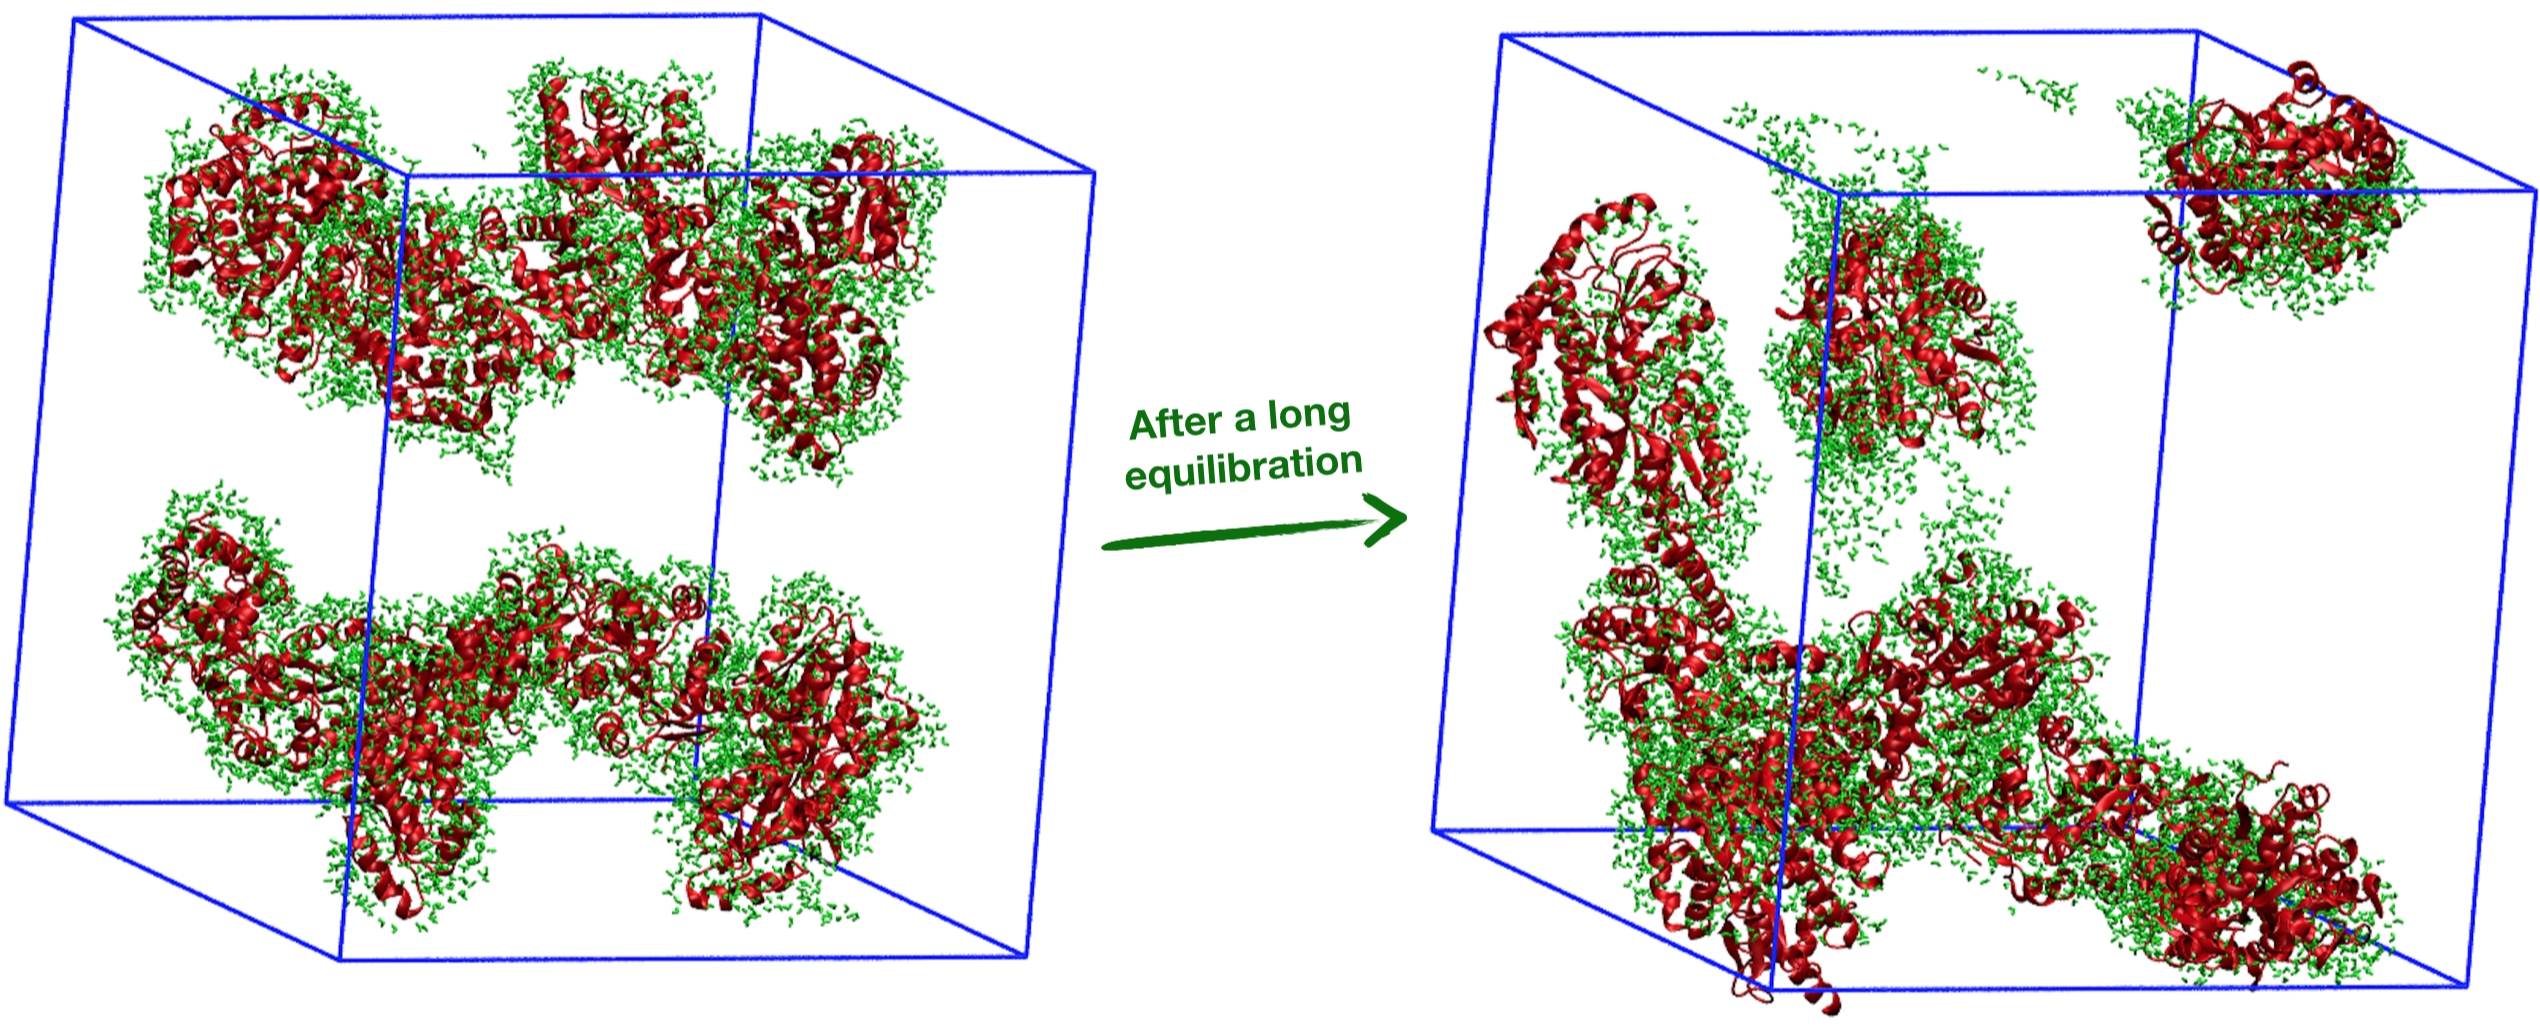
\includegraphics[width=\textwidth]{pbc-1omp-cube-wrongbox02.jpg}
    
    \footnotesize{\caption{Example of a large box containing a MBP in a poor hydrated solution. After several time simulations, alternating phases of heating in NVT and equilibration in NPT, the final state is still physically unacceptable. \textit{Picture realized with VMD.}}
    \label{fig:wrong-hydr}
    }
\end{minipage} 
\end{figure}

These type of complications imply that even if real experiments are performed in powder samples, very often, hydrated systems are however simulated for simplification. For example, in 2004, Balog et al. made an experiment of neutron scattering and showed that a particular protein in the holo form vibrates more intensively at lower frequencies (between 50 and 500 GHz) compared to the same protein in the apo form.
In 2011, also Balog along with other colleges, performed a series of MD simulations to deepen the analysis of the previously studied systems. Even if the interesting results collected were a product of the analysis of simulations that represented much more hydrates solutions from those studied with neutrons.
%Questo tipo di complicazione fa si che, anche se si svolgono esperimenti reali su campioni in polvere, molto spesso si simulano comunque sistemi idratati. Ad esempio, nel 2004, Balog et al. fecero un esperimento di neutron scattering e mostrarono che una patricolare proteina nella forma holo vibra più intensamente alle basse frequenze (fra $500$ e $50$ GHz) rispetto alla stessa proteina nella forma apo. Nel 2011, sempre Balog insieme ad altri colleghi, realizzò una serie di MD simulazioni per approfondire l'analisi dei sistemi studiato precedentemente. Sebbene i risultati interessanti che ottenerro, di fatto nelle loro simulazioni vennero fatti evolvere dinamicamente dei sistemi che di fatto rappresentavano soluzioni molto più idratate di quelle studiate con i neutroni.\footnote{Per ovviare a questo, dopo l'evoluzione dinamica dei sistemi abbondantemente idratati, rimossero l'acqua in eccesso ed effettuarono una minimizzazione localizzata dell'energia utilizzando the ABNR (adopted basis Newton Raphson) method -- a minimization method applied in a small subspace of the molecule.}

The methodology used by Balog et al., initially developed by Loncharichi R. J. and Brooks B. R. \cite{loncharich1990temperature}, allows in fact to obtain barely accurate information to study the internal dynamics of the proteins, however is not adapted to study the properties of the hydrating water that surrounds the protein, of barely hydrated solutions \cite{tarek2000dynamics}.
%La metodologia utilizzata da Balog e colleghi, sviluppata inizialmente da Loncharichi R. J. and Brooks B. R. \cite{loncharich1990temperature}, permette infatti di ottenere informazioni abbastanza accurate per studiare la dinamica interna delle proteine, ma si adatta male per studiare le proprietà dell'acqua di idratazione che circonda le proteine in queste soluzioni poco idratate \cite{tarek2000dynamics}. 

On the other hand, it is possible to solve the problems raised from the low hydration, by simulating eight instead of only one protein \cite{tarek2000dynamics}. In this way, even if the computational cost is much more elevated, it is possible to reduce the volume of the box at its most, without risking that a protein interacts with itself. Even if also in this case, the possibility that empty regions are created is still very high, due to the irregular configuration of the protein. In fact, it is very difficult to find a configuration that is compact enough to prevent the formation of hole and, at the same time, where there is no overlapping among the atoms of the proteins. One of the greatest difficulties consists in positioning three-dimensionally, all eight proteins to obtain a well enough initial state.
%D'altra parte, è possibile risolvere i problemi dovuti alla bassa idratazione simulando otto proteine invece che una sola \cite{tarek2000dynamics}. In questo modo, infatti, anche se ovviamente il costo computazionale risulta più elevato, è possibile ridurre il volume della box il più possibile senza rischiare che una proteina interagisca con se stessa. Tuttavia, la possibilità che si creino dei vuoti fra le proteine è ancora molto elevata. A causa della forma irregolare delle proteine, infatti, diventa molto difficile trovare una configurazione compatta abbastanza da impedire la formazione di hole e in cui, allo stesso tempo, ci siano delle sovrapposizioni fra gli atomi delle proteine. Una delle maggiori difficoltà consiste proprio nel disporre tridimensionalmente le otto proteine per ottenere un buono stato iniziale. \\

%!!!!!!!!!!!!
%Per questo motivo, simulazioni di proteine in polvere in letturatura sono molto poche. Un punto di riferimento importante è l'articolo di Tarek M. e Tobias D. J.: ``\textit{The Dynamics of Protein Hydration Water: A Quantitative Comparison of Molecular Dynamics Simulations and Neutron-scattering Experiments}'' where the authors present an extensive molecular dynamics simulation study of protein hydration water, at a series of temperatures in cluster, crystal, and powder environments \cite{tarek2000dynamics}.

Therefore, simulations of proteins in powders in the literature are scarce. One of the most important references is the article by Tarek M. and Tobias D. J.: ``\textit{The Dynamics of Protein Hydration Water: A Quantitative Comparison of Molecular Dynamics Simulations and Neutron-scattering Experiments}'' where the authors present an extensive molecular dynamics simulation study of protein hydration water, at a series of temperatures in cluster, crystal, and powder environments \cite{tarek2000dynamics}.

If we take into account what has been studied by Tarek and Tobias, generally what is done to simulate powder systems is to replicate eight times the structure of the protein and to arrange these structures on the vertex of the unit cell of the crystal sample which has been used to determine the structure of the primary protein\footnote{Usually, this information is contained in the PDB file of the protein, available in the Protein Data Bank (see section \ref{sssec:PDB}).}. In this way, it is obtained a pseudo-crystall that, as shown by Tarek and Tobias, represents a good starting point to develop MD simulations of powdery systems. Afterwards, the correct quantity of water around the eight proteins is added, carefully paying attention to not leaving empty regions in the box.

%Seguendo quanto fatto da Tarek e Tobias quello che in genere si fa per simulare sistemi in polvere è di replicare otto volte la struttura di una proteina e disporre nello spazio le varie copie della proteina ai vertici della cella unitaria del crystal lattice del campione che è stato utilizzato per determinare la struttura della proteina di partenza\footnote{solitamente questa informazione è contenuta nel file PDB della proteina ricavabile dal sito del Protein Data Bank -- vedi sezione \ref{sssec:PDB}.}, ottenendo di fatto uno pseudo-cristallo che, come hanno dimostrato Tarek e Tobias, rappresenta un buon punto di partenza per svilluppare MD simulazioni di sistemi in polvere. Dopo di che si aggiunge la giusta quantità d'acqua intorno alle otto proteine, cercando i non lasciare spazi vuoti.

\subsection{The initial state of the simulations}
The main programs used for this phase were: NAMD \cite{ref:NAMD} and VMD \cite{humphrey1996vmd} and several original scripts were written in tcl language. The principal steps performed to obtain the initial configurations of the multiple systems were:
%Il programma principalemnte utilizzati in questa fase sono stati: NAMD \cite{ref:NAMD} and VMD \cite{humphrey1996vmd} e per ottenere la configurazione iniziale dei vari sistemi diversi script originali in tcl sono stati scritti. In particolare, i passi principali che sono stati messi in pratica sono:
\begin{itemize}
\item \textbf{Getting the PDB files}\\
The (.pdb) files representing the three-dimensional structures of the systems that are to be studied were retrieved from the site: \url{http://www.rcsb.org/}. The selected files were, respectively, \textit{1omp.pdb} for MBP \cite{sharff1992crystallographic} and \textit{1anf.pdb} for MBP+Malt \cite{quiocho1997extensive}.
%Sul sito \url{http://www.rcsb.org/} si sono per individuati i files .pdb ottenuti tramite X-ray crystallography che rappresentano le strutture tridimensionali dei sistemi che si intende studiare. Rispettivamente, \textit{1anf.pdb} per MBP+Malt \cite{quiocho1997extensive} e \textit{1omp.pdb} per MBP \cite{sharff1992crystallographic}.
%\begin{center}
%{\large \textbf{CHRYSTAL STRUCTURES}}
%\end{center}
\vspace{-0.25cm}
\begin{figure}[h]
\begin{center}
\begin{minipage}[t]{0.9\textwidth}
\centering
\hspace{0.75cm}
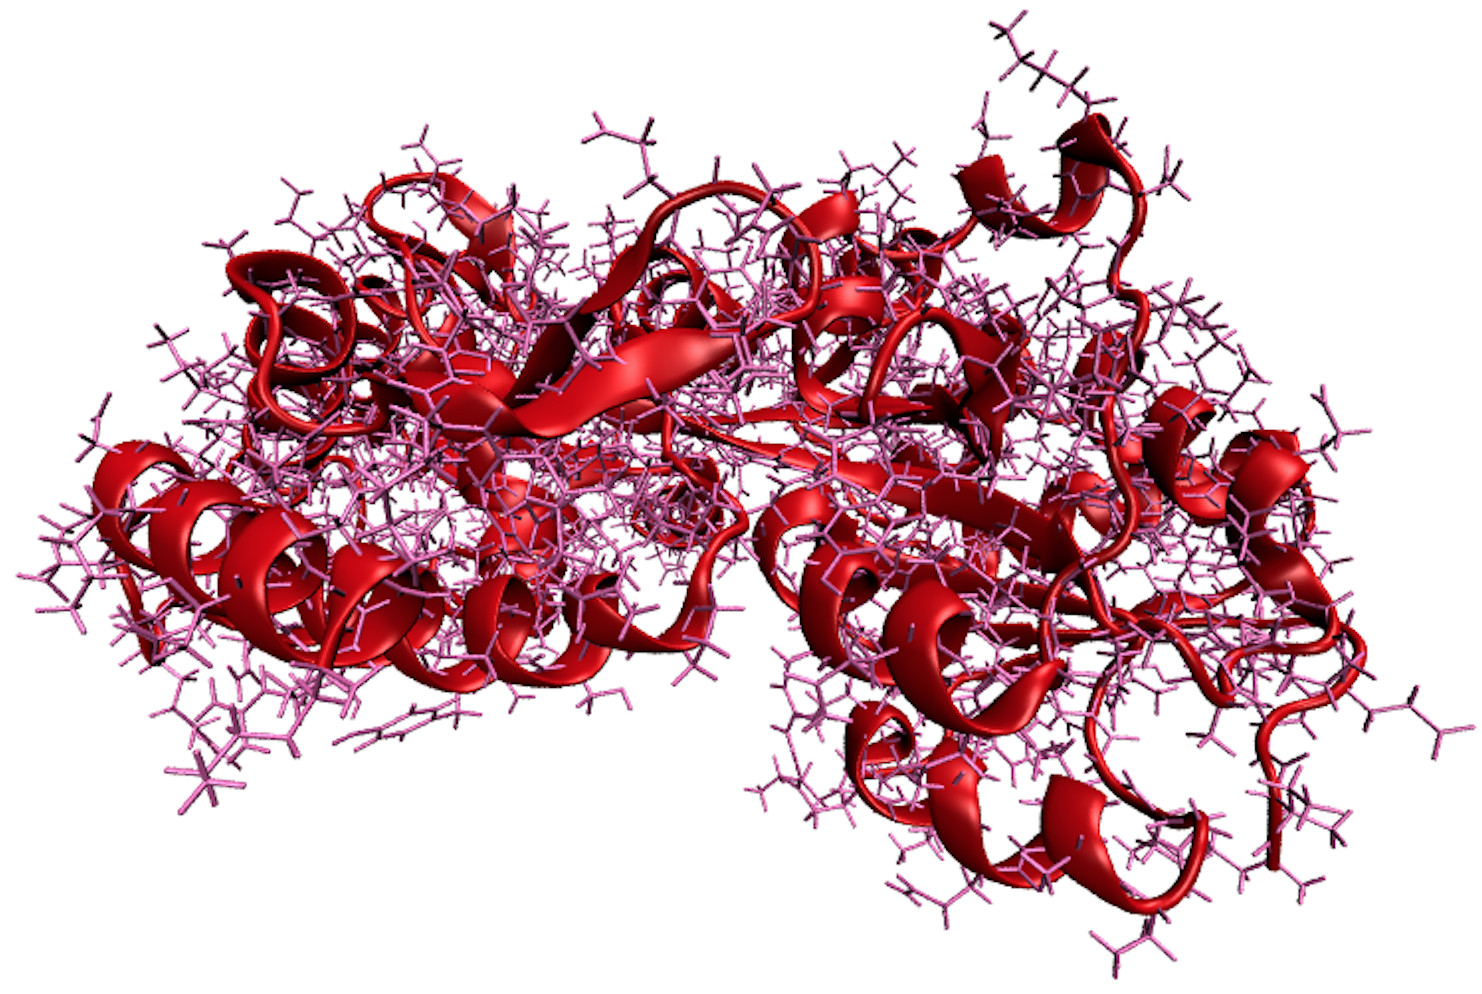
\includegraphics[width=0.45\textwidth]{mbp.jpg}
\hspace{0.2cm}
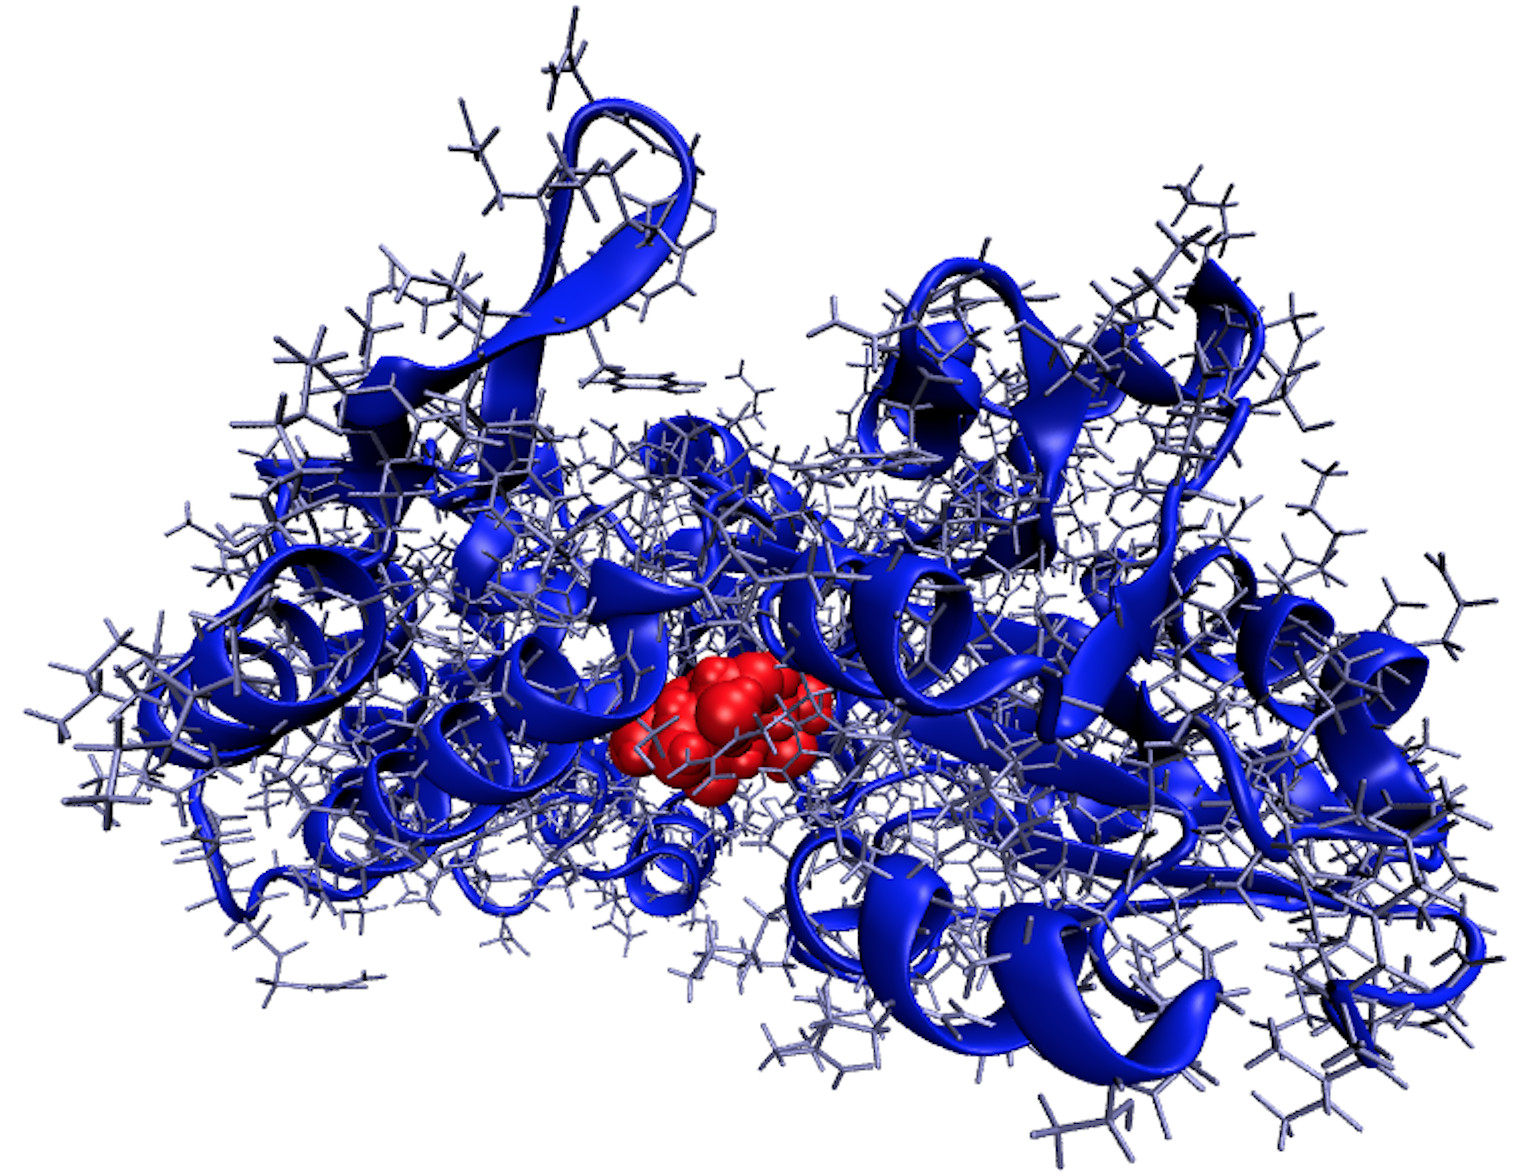
\includegraphics[width=0.45\textwidth]{mbp+malt.jpg}
\end{minipage} 

\hspace{1.65cm}
\textbf{MBP}
\hspace{4.75cm}
\textbf{MBP+Maltose}

\hspace{0.6cm}
\textbf{(}\small{PDB code: 1omp}\textbf{)}
\hspace{3.8cm}
\textbf{(}\small{PDB code: 1anf}\textbf{)}
\end{center}

\vspace{-0.25cm}
    \footnotesize{\caption{Chrystal structures of the studied system. \textit{Picture realized with VMD.}}
    \label{fig:pdb-structures}
    }
\end{figure}

\item \textbf{Generating the PSF files}\\
Using the \textit{psfgen} package of VMD, brief scripts in tcl language were implemented that allow to create the (.psf) file of each system from their (.pdb) file. Moreover, during this phase, the coordinates of the hydrogen atoms were added. Indeed, in the structures described in the (.pdb) file downloaded from the web, the hydrogen atoms were missing because those structures were obtained by X-ray crystallography. The (.top) files used, were the ones related to forcefield CHARMM36 that was decided to use for the simulations -- they were downloaded from the site: \url{http://mackerell.umaryland.edu/charmm_ff.shtml}. 

\item \textbf{Building the 3D arrangement of the 8 proteins in a powder}\\
Initially, as it is usual in powder system simulations \cite{rahaman2017configurational, fichou2015molecular}, an attempt to arrange the eight proteins in the vertex of the unit cell indicated in the files \textit{1anf.pdb} and \textit{1omp.pdb} was made. In both cases, the original samples were triclinic crystal and this would have implied a complication in the data analysis for taking into account the periodic conditions -- in a triclinic crystal the vectors of the unit cell are of unequal length and the angles between them are all different, hence the boundary conditions applied on such systems are more complex than those usually applied on orthorhombic crystal\footnote{For orthorhombic crystals, the angles between the vectors of the unit cell are all of 90$^\circ$}. Furthermore, in the \textit{1anf.pdb} (MBP+Malt), the dimensions of the unit cell were bigger with respect to the protein dimensions and this would have lead to the problematic described in the first scenario of the previous section.
\begin{figure}[h]
\begin{center}
\begin{minipage}[t]{0.9\textwidth}
\centering
\hfill
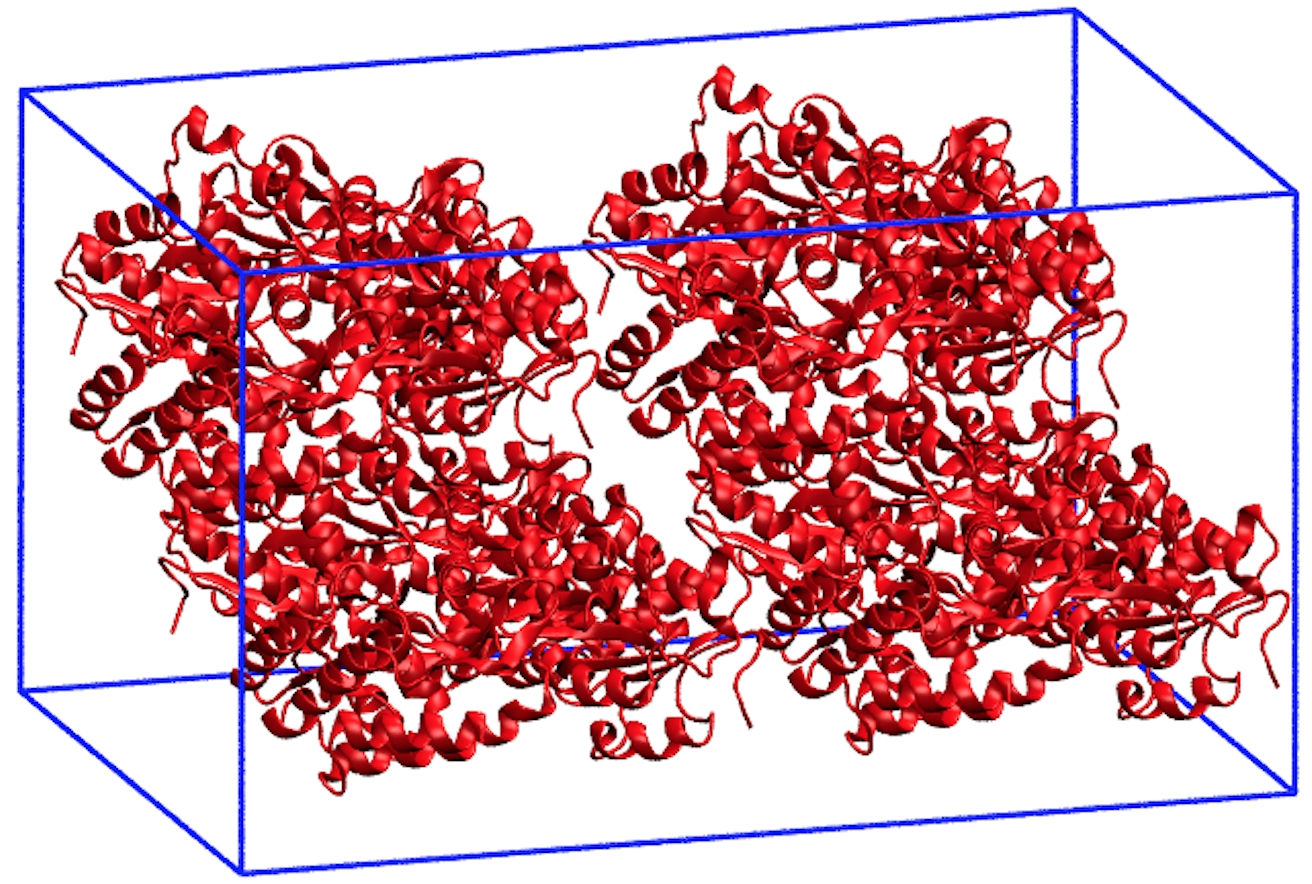
\includegraphics[width=0.45\textwidth]{1anf-l8.jpg}
\hspace{0.65cm}
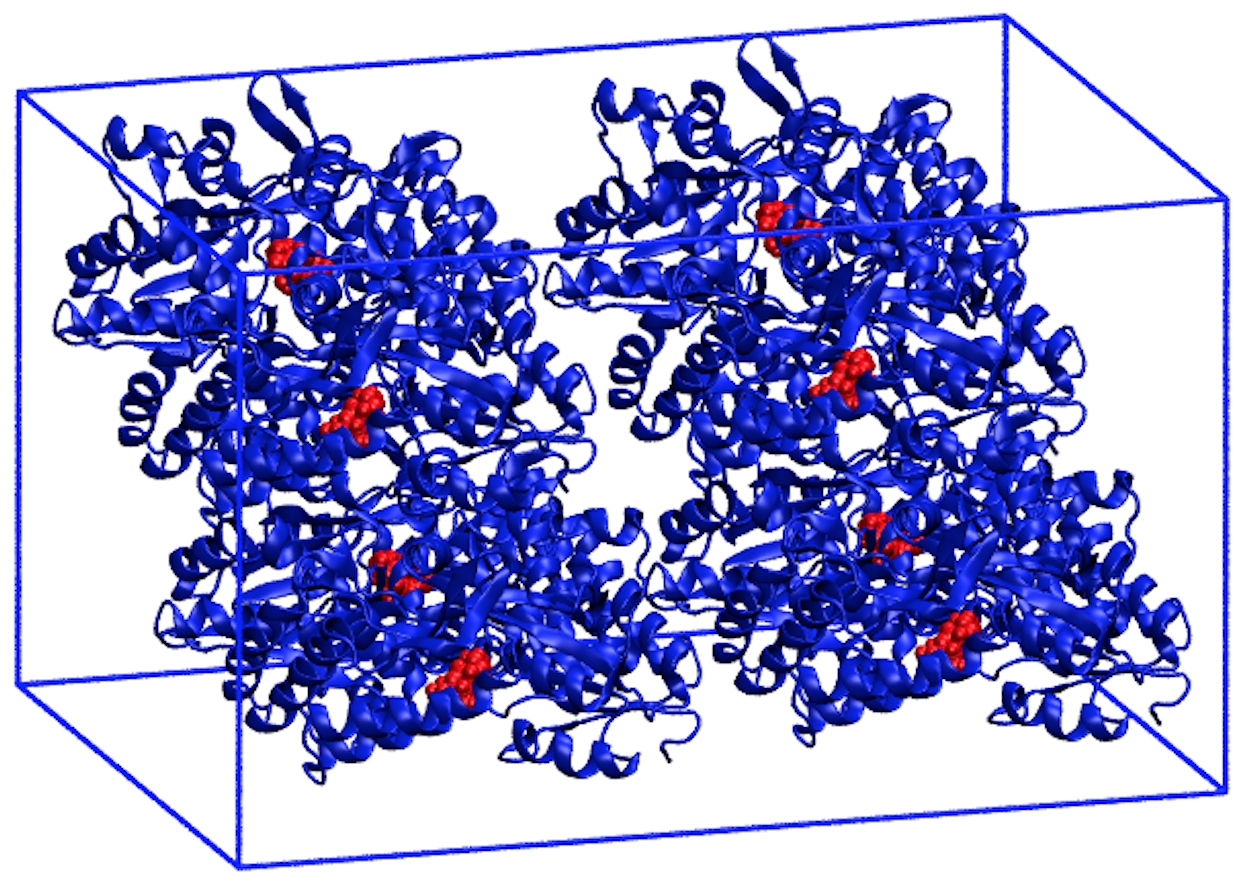
\includegraphics[width=0.45\textwidth]{1omp-l8.jpg}
\hfill
\end{minipage} 

\hspace{1.5cm}
\textbf{MBP}
\hspace{4.75cm}
\textbf{MBP+Maltose}

    \footnotesize{\caption{3D arrangement of the proteins in two studied systems. \textit{Picture realized with VMD.}}
    \label{fig:protein-box}
    }
\end{center}
\end{figure}

%Inizialmente, as usual for simulations of powder systems \cite{rahaman2017configurational}, si è provato a posizionare le otto proteine ai vertici della celle unitarie dei crystal lattices indicati, rispettivamente, nei file \textit{1anf.pdb} e \textit{1omp.pdb}. In entrambi i casi, i sistemi studiati con la cristallografia erano dei triclinic crystal e questo avrebbe comportato una complicazione nell'analisi dati per tenere conto delle condizioni periodiche -- in a triclinic crystal the vectors of the unit cell are of unequal length and the angles between them are all different, hence the boundary conditions applied on these systems are more complex than those usually applied on orthorhombic crystal\footnote{For orthorhombic crystals, the angles between the vectors of the unit cell are all of 90$^\circ$}. Per di più, in \textit{1anf.pdb} (MBP+Malt), la dimensione della cella unitaria era molto grande rispetto alla dimensione dela proteina e questo avrebbe portato alla condizione problematica descritta nel primo scenario nella sezione precedente.\\
Therefore, considering that powders are actually highly disordered and hence do not present a real crystal structure, to solve these problems, the eight proteins were arranged in an arbitrary configuration, chosen to get an orthorhombic box with the proteins packed as mush as possible. In order to achieve this, several scripts were implemented to relocate and rotate the various proteins, so that in the end, using the package \textit{topotools} of VMD \cite{vmd-topotools}, the following files could be created:
%Quindi, considerando che in realtà le polveri sono altamente disordinate e non presentano una vera struttura cristallina, si è pensato di posizionare le otto proteine in una configurazione arbitraria che è scelta in modo da avere una box di orthorhombic shape e un sistema il più compatto possibile. Per fare questo si sono implementati vari script per spostare e ruotare le diverse proteine, così da crare alla fine, utilizzando il pacchetto \textit{topotools} di VMD \cite{vmd-topotools}, i files:
\begin{itemize}
\item[$\triangleright$] \textit{1anf-l8.pdb} and \textit{1anf-l8.psf} -- positions and structure of the MBP+Malt systems.
\item[$\triangleright$] \textit{1omp-l8.pdb} and \textit{1omp-l8.psf} -- positions and structure of the MBP systems.
\end{itemize}
In any case, finding an optimal configuration is quite complicated, in fact, several attempts were needed to find the right configuration in the end. The final configuration is shown in Fig. \ref{fig:protein-box}.

\item \textbf{Adding water}\\
The values of hydration $h$ selected to simulate both systems, were chosen to allow, in the future, to use the results collected by Paciaroni and colleagues, which measurements were made with neutrons, their results have not yet been published. In this sense, the MBP+Malt hydration value was established at $h = 35.6\%$  (which corresponds to circa 6,488 molecules of water) and MBP with $h = 34.8\%$ (which would represent 6,289 molecules of water).
Thus, the simulated systems may provide not only interesting information from the beginning, but can also be used in the future to analyze in detail the results obtained with the neutrons.\\
%Per i valori di idratazione dell'idratazione $h$ da ricreare per i due sistemi, si è deciso di simulare MBP+Malt con $h = 35.6\%$ (corrispondente a circa 6,488 molecole di acqua) e MBP con $h = 34.8\%$ (corrispondente a  6,289). Questi valori sono stati scelti per permettere, in futuro, di utilizzare le simulazioni realizzate nel corso del presente lavoro per analizzare in dettaglio i risultati di alcune misure fatte con i neutroni by Paciaroni and colleges, not yet published. In questo modo i sistemi simulati, non solo forniranno fin da subito nuove informazioni, ma potranno anche essere utilizzati in futuro per analizzare in dettaglio i risultati delle misure fatte con i neutroni.\\
Specifically, to add water to the systems, some tcl scripts were realized using the packages: \textit{solvate}, \textit{psfgen} and \textit{topotools} of VMD. For each one of the systems a box filled with water was created in such a way, that it would contain all eight proteins and to leave 6 $\AA$ of distance between the proteins and the surfaces of the box. In this way the molecules of water, located randomly in the box surrounded entirely the protein. Nevertheless, the number of water molecules added in both systems were more than the ones needed to obtain the desired quantity of hydration. For this reason, after adding the water, the H$_2$O molecules with a distance greater than a fixed quantity $x$ from their nearest protein were removed. Changing the value of the $x$, change the total number of H$_2$O still in the box. Hence, for each one of the systems, a certain $x$ was selected to obtain the number of water molecules required. This was possible because the starting configurations \textit{1anf-l8.pdb} and \textit{1omp-l8.pdb} were compact enough and therefore, even after the removal of some water molecules no empty regions of great dimensions were created between the proteins. The results, saved in \textit{1anf-hyd.pdb} and \textit{1omp-hyd.pdb} (and the associated PSF files) are displayed in Fig. \ref{fig:water-box}.
%Nello specifico, per aggiungere l'acqua ai sistemi, sono stati implementati alcuni script in tcl utilizzando i pacchetti: \textit{solvate}, \textit{psfgen} and \textit{topotools} di VMD. In particolare, per ognuno dei due sistemi si è creata una box piena d'acqua tale da contenere tutte e otto le proteine e da lasciare 6$\AA$ di distanza fra le proteine e le superfici della box. In questo modo le molecole d'acqua posizionate casualemente hanno circondato completamente le proteine. Tuttavia, il numero di molecole d'acqua aggiunte in questo modo nei due sistemi è risutlato troppo elevato rispetto al numero di molecole d'acqua necessarie per ottenere le idratazioni volute. Per questo motivo, dopo aver aggiunto l'acqua, si provveduto a rimuovere le molecole di H$_2O$ distanti più di una certa quantità $x$ dalle proteine. Per ognuno dei due sistemi, si è scelta perciò una $x$ tale da ottenere il numero di molecole d'acqua richiesto. Questo è stato possibile proprio grazie al fatto che le configurazioni di partenza \textit{1anf-l8.pdb} e \textit{1omp-l8.pdb} erano molto compatte e quindi, anche dopo aver rimosso le molecole d'acqua non si sono creati regioni vuote fra le proteine di dimensioni eccessive. I risultati, salvati in \textit{1anf-hyd.pdb} e \textit{1omp-hyd.pdb} (più i relativi file PSF associati) sono mostrati in Fig. \ref{}

\begin{figure}[h]
\begin{center}
\begin{minipage}[t]{0.9\textwidth}
\centering
\hfill
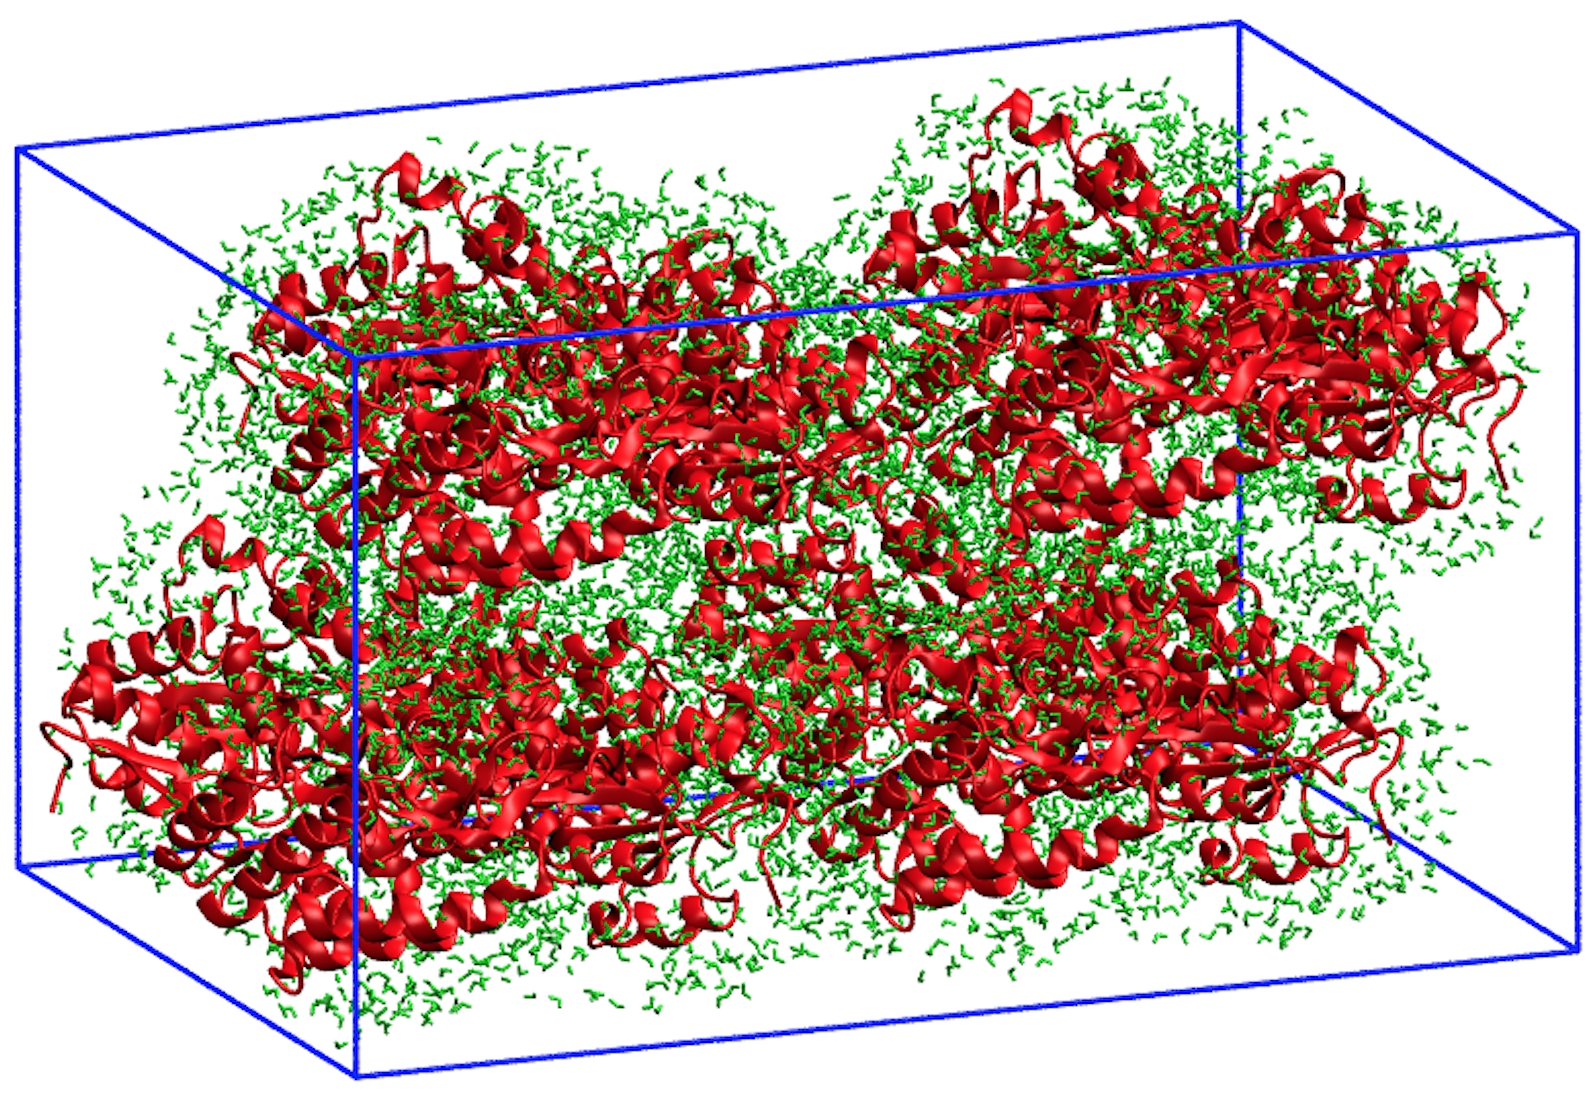
\includegraphics[width=0.45\textwidth]{1omp-hyd.jpg}
\hspace{0.5cm}
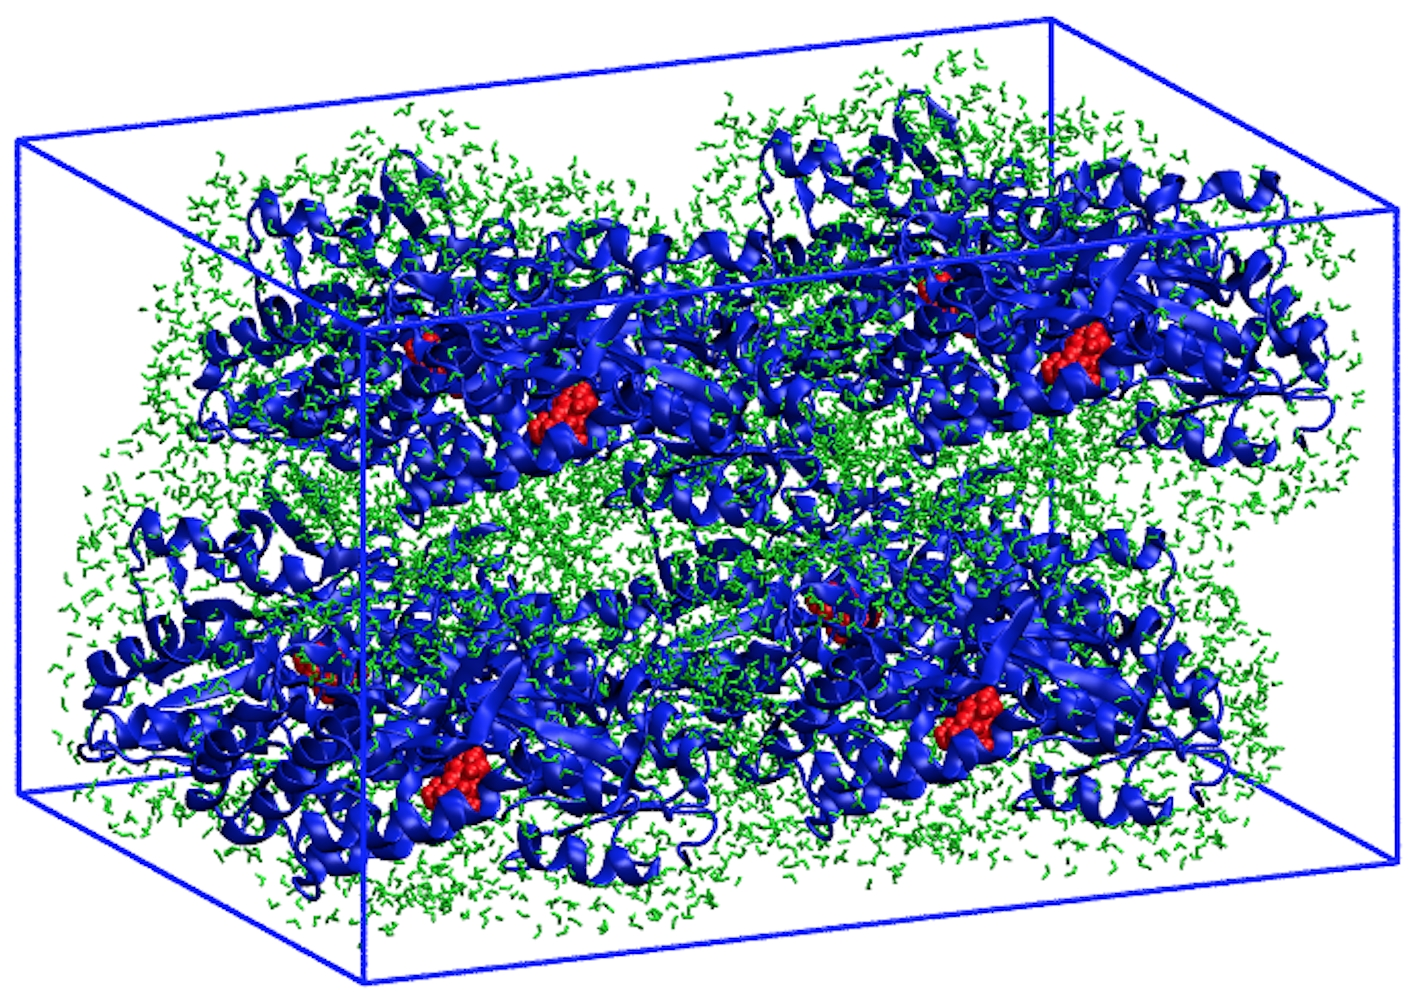
\includegraphics[width=0.45\textwidth]{1anf-hyd.jpg}
\hfill
\end{minipage} 

\hspace{1cm}
\textbf{MBP}
\hspace{4.75cm}
\textbf{MBP+Maltose}

    \footnotesize{\caption{Box of the two systems after the adding of water. \textit{Picture realized with VMD.}}
    \label{fig:water-box}
    }
\end{center}
\end{figure}

\item \textbf{Adding ions}\\
Finally, due to the presence of residues electrically charged in the MBP that do not balance entirely in the system, the protein exhibit a net electric charge. Precisely, the charged residues in an MBP are: 37 Lys (+), 27 Glu (-), 24 Asp (-), 6 Arg(-); hence the MBP has an electric charge of -8. To restore the electrical neutrality of the simulated systems, it was necessary to add ions to the water solution. This was possible using the \textit{autoionize} package of VMD. The structures obtained in this way, can be used to start the energy minimization phase.
%Alla fine, a causa della presenza di residui carichi elettricamente nella MBP che non si bilanciano completamente si riscontra che proteina presenta una carica elettrica complessiva pari a -8. Nello specifio, i resiudui carichi in una MBP sono: 37 Lys (+), 27 Glu (-), 24 Asp (-), 6 Arg(-). Pertanto per rendere neutri i sistemi simulati è stato necessario aggiungere degli ioni alle soluzioni acquose. Questo è stato fatto utilizzando il pacchetto \textit{autoionize} di VMD. Le strutture ottenute sono possono essere così utilizzate per iniziare la fase di minimizzazione nell'energia.

\item \textbf{Minimization}\\
In this phase NAMD were largely employed. The forcefield adopted was CHARMM36 and the main parameters set in the \textit{config} file, for both systems, were\footnote{As a reference of the NAMD commands see ``\textit{NAMD User's guide}'' retrievable at \url{https://www.ks.uiuc.edu/Research/namd/2.12/ug.pdf} \cite{ref:NAMD_ug}}:\\
%In questa fase si iniziato ad utilizzare NAMD. Il forcefield utilizzato è CHARMM36 ed i principali parametri impostati nel \textit{config} file, per entrambi i sistemi, sono\footnote{Come riferimento al significato dei vari comandi si rimanda alla ``\textit{NAMD User's guide}'' reperibile sul sito \url{https://www.ks.uiuc.edu/Research/namd/2.12/ug.pdf} \cite{ref:NAMD_ug}}:\\
\begin{center}
\textbf{Forcefield parameters:}
\vspace{-0.25cm}
\begin{equation*}
\begin{array}{ll}
\text{\textit{exclude:}} \qquad\quad & \text{scaled1-4}\\
\text{\textit{1-4scaling:}} \qquad\quad & 1.0\\
\text{\textit{cutoff:}} \qquad\quad & 10.0\\
\text{\textit{switching:}} \qquad\quad & on\\
\text{\textit{switchdist:}} \qquad\quad & 9.0\\
\text{\textit{pairlistdist:}} \qquad\quad & 12.0\\
\end{array}
\end{equation*}
\end{center}
The number of steps for the minimization process are set as 5,000. As shown in Fig. \ref{fig:energy-min}, this number of steps is enough to achieve a quite stable local minimum, indeed, an increase of the number of steps would not produce a significant decrease in the total energy.
%Il numero di steps per la minimizzazione è stato impostato a 5,000. Come si può vedere dalla Fig. \ref{}, questo numero di steps è sufficiente a raggiungere un minimo locale sufficientemente stabile, infatti anche se si aumentasse ulteriormente il numero di steps non si otterrebbe una diminuzione significativa dell'energia totale.\\

\begin{figure}[H]
\centering
\begin{minipage}[t]{0.775\textwidth}
	\centering
    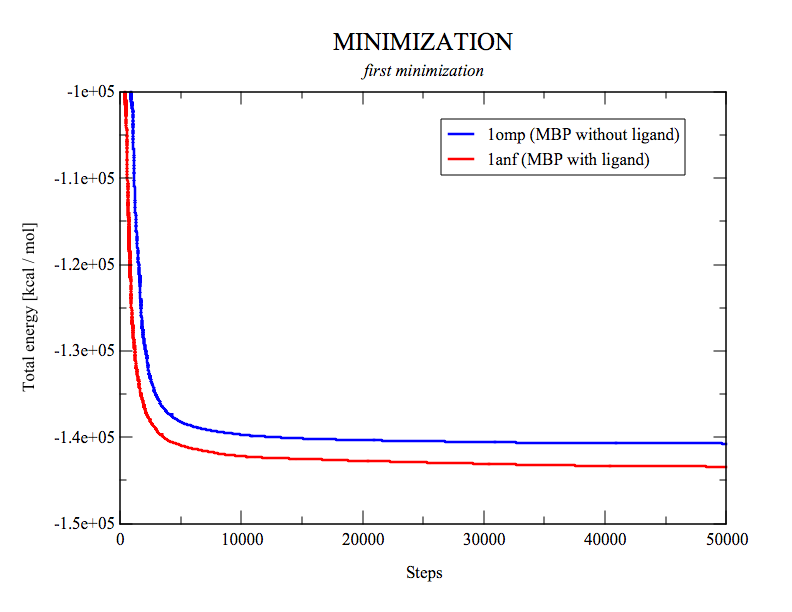
\includegraphics[width=0.95\textwidth]{first-minimization.png}
    
    \footnotesize{\caption{Results of the energy minimization. \textit{Picture realized with QtGrace.}}
    \label{fig:energy-min}
    }
\end{minipage} 
\end{figure}


\item \textbf{Heating and NPT equilibration}\\
The real dynamic evolution of the system starts in this phase. To achieve an acceptable state of the system at 300 K a series of simulations at 1 $ns$ were performed, alternating heating in NVT and NPT equilibration. The intermediate temperatures for the heating process were: 60 K, 120 K, 180 K, 240 K, 270 K, 285 K, 300 K. The main parameters in the \textit{config} files for this simulations were set as shown in the following tables\footnote{The forcefield parameters were the same as the ones for the minimization.}:
%In questa fase inizia la vera e propria evoluzione dinamica del sistema. Per arrivare ad una ad avere i sistemi in un buono stato a 300K si sono effettuata una serie di simulazioni di 1 $ns$ ciascuna dove si sono alterante fasi di heating in NVT e equilibrature in NPT. Le temperature intermedie sono state: 60 K, 120 K, 180 K, 240 K, 270 K, 285 K, 300 K. I parametri principali impostati nei \textit{conifg} files, per queste simulazioni, sono stati\footnote{I parametri per il forcefield sono stati lasciati uguali a quelli impostati per la minimizzazione.}:
%\begin{center}
%\begin{minipage}{0.45\textwidth}
%\begin{center}
%\textbf{Integrator parameters:}
%\vspace{-0.25cm}
%\begin{equation*}
%\begin{array}{ll}
%\text{\textit{timestep:}} \qquad\quad &1.0\\
%\text{\textit{rigidBonds:}} \qquad\quad & \text{all}\\
%\text{\textit{nonbondedFreq:}} \qquad\quad & 1\\
%\text{\textit{fullElectFrequency:}} \qquad & 2\\
%\text{\textit{steppercycle:}} \qquad & 10\\
%\end{array}
%\end{equation*}
%\end{center}
%\end{minipage}
%\begin{minipage}{0.45\textwidth}
%\begin{center}
%\vspace{-1.55cm}
%\textbf{PME (Particle-Mesh Ewald)}
%\vspace{-0.25cm}
%\begin{equation*}
%\begin{array}{ll}
%\text{\textit{PME:}} \qquad\quad & \text{yes}\\
%\text{\textit{PMEGridSpacing:}} \qquad\quad & 1.3\\
%\end{array}
%\end{equation*}
%\end{center}
%\end{minipage}
%\end{center}
%
%\begin{center}
%\textbf{MBP (\textit{1omp})\\Periodic boundary conditions -- unit cell:}
%\vspace{-0.25cm}
%\begin{equation*}
%\begin{array}{lrrr}
%\text{\textit{cellBasisVector1:}} \qquad\quad & 97.0 \qquad & 0.0 \qquad & 0.0\\
%\text{\textit{cellBasisVector2:}} \qquad\quad & 0.0 \qquad & 80.0 \qquad & 0.0\\
%\text{\textit{cellBasisVector3:}} \qquad\quad & 0.0 \qquad & 0.0 \qquad & 142.0\\
%\text{\textit{cellOrigin:}} \qquad & 0.0 \quad & 0.0 \quad & 0.0\\
%\end{array}
%\end{equation*}
%
%\textbf{MBP+Malt (\textit{1anf})\\Periodic boundary conditions -- unit cell:}
%\vspace{-0.25cm}
%\begin{equation*}
%\begin{array}{lrrr}
%\text{\textit{cellBasisVector1:}} \qquad\quad & 97.0 \qquad & 0.0 \qquad & 0.0\\
%\text{\textit{cellBasisVector2:}} \qquad\quad & 0.0 \qquad & 80.0 \qquad & 0.0\\
%\text{\textit{cellBasisVector3:}} \qquad\quad & 0.0 \qquad & 0.0 \qquad & 142.0\\
%\text{\textit{cellOrigin:}} \qquad & 0.0 \quad & 0.0 \quad & 0.0\\
%\end{array}
%\end{equation*}
%\end{center}
\begin{figure}[H]
\hfill
\begin{minipage}[t]{0.925\textwidth}
	\centering
    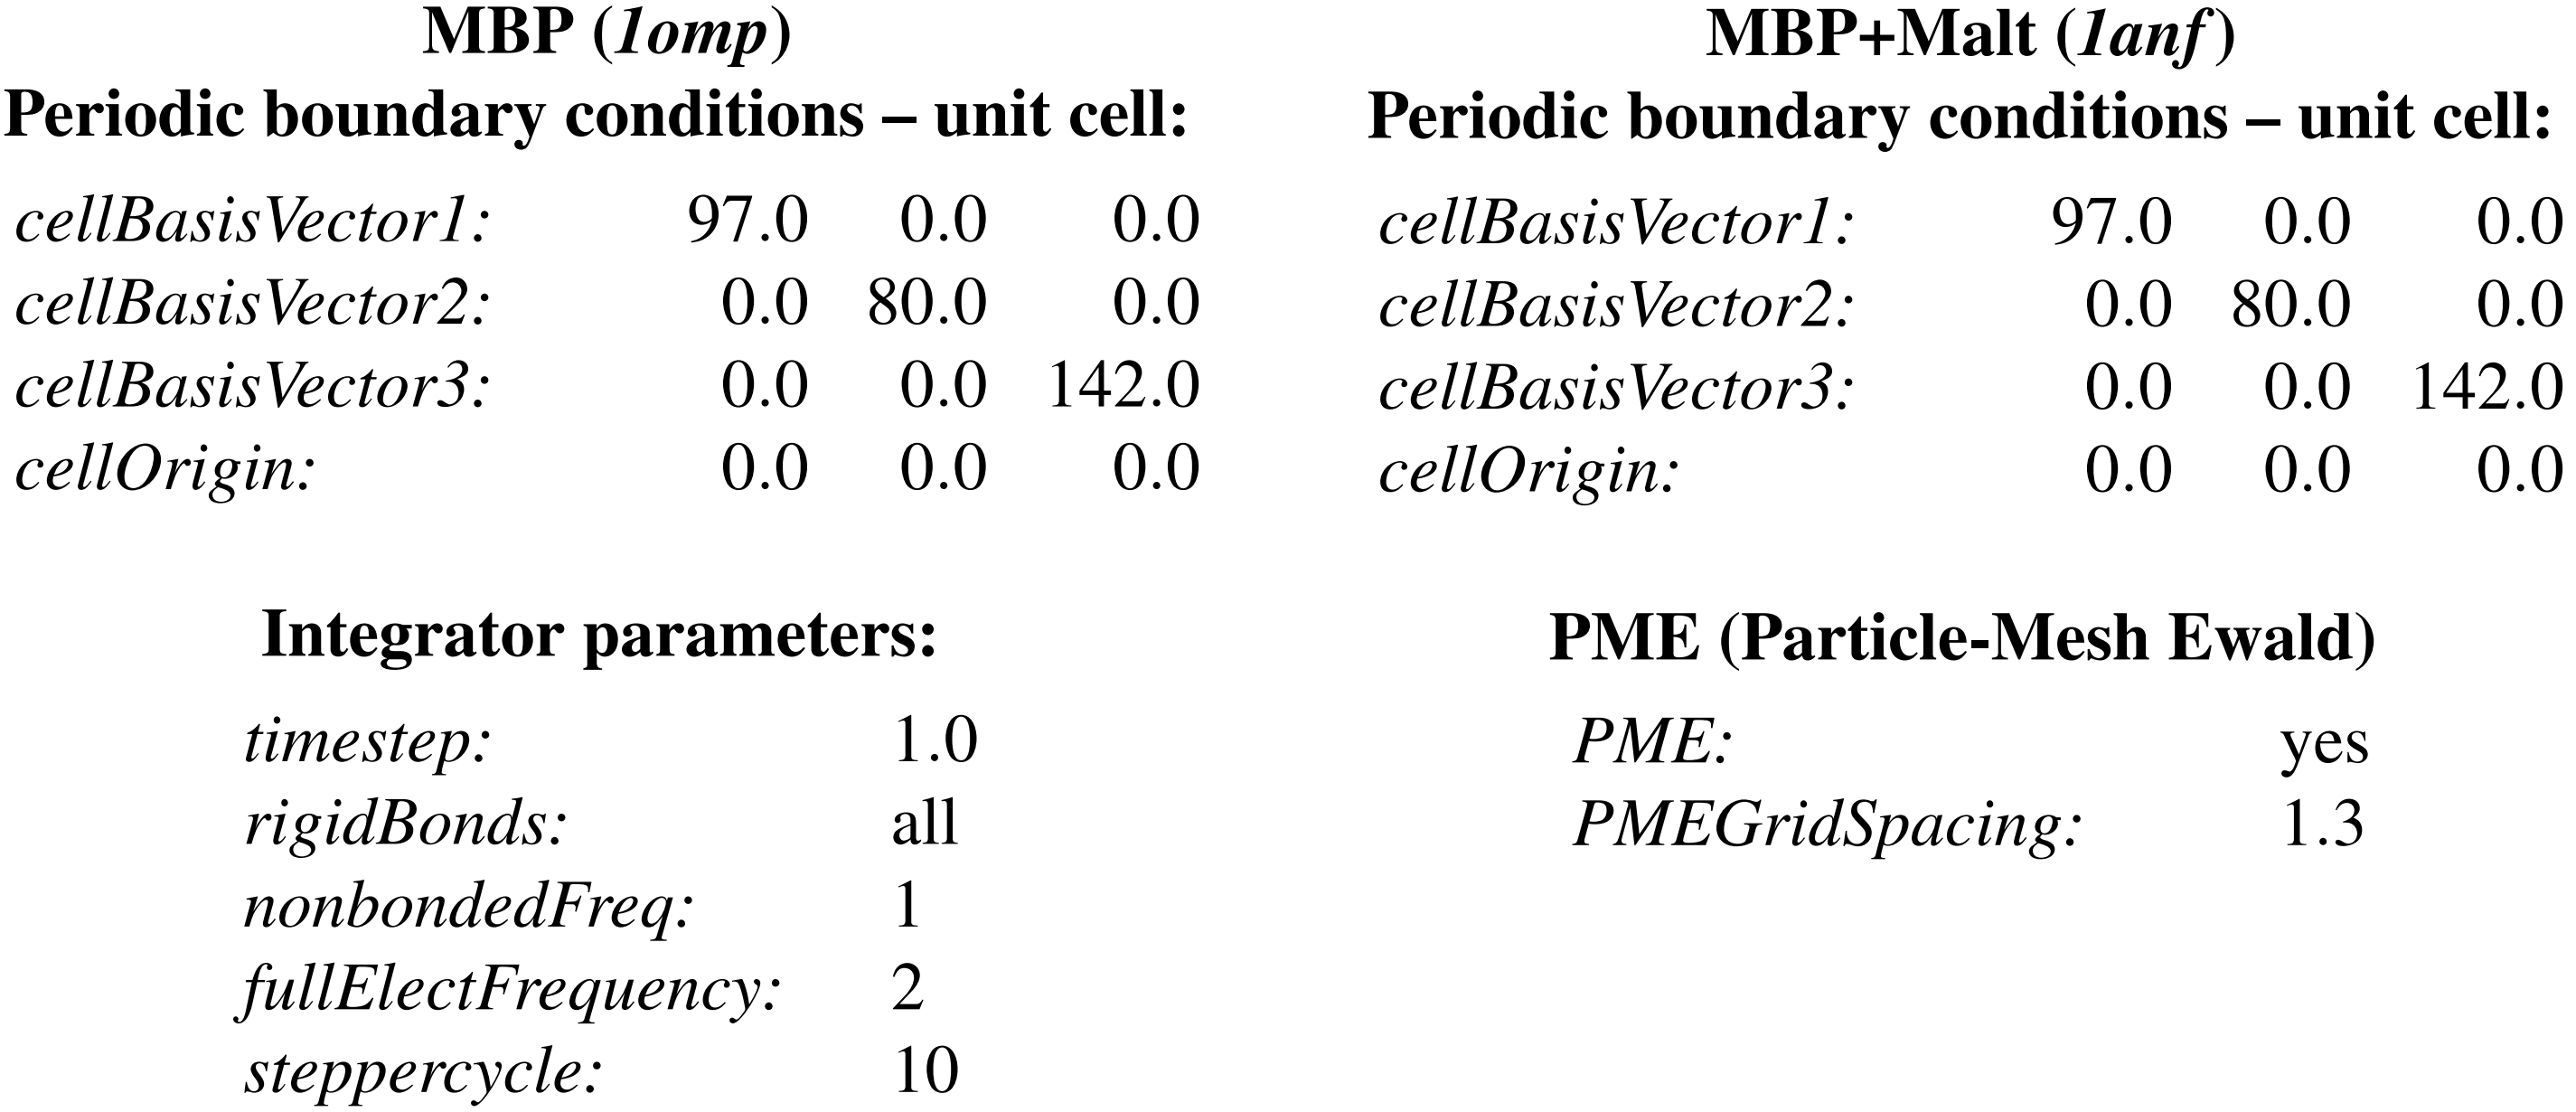
\includegraphics[width=\textwidth]{parameters3.png}
\end{minipage} 
\end{figure}


The results of these simulations for the MBP system are reported in graphs and pictures. The graphs show the energy and the volume of the simulated system as a function of the time. The pictures report three frames drawn from the simulations, representing a sort of summary of the evolution of the MBP system during the heating (in last picture, the simulation box is replicated using two periodic images). As one can observe, at the end of the simulations, the configuration assumed by the system is reasonably packed and does not display any empty regions, thus it provides a good starting point for simulations of the MBP powder. The results obtained for the MBP+Malt system are not displayed in this section, because they are similar to those of the MBP system. \\
%Il risultato di queste simulazioni per il sistema MBP è riportato nelle Fig. \ref{} dove sono mostrati i grafici dell'andamento dell'energia e del volume durante queste simulazioni e Fig. \ref{} dopo è mostrato una sorta di riassunto della simulazione da due angolazioni diverse. Come si può vedere, alla fine di questa fase, la configurazione assunta dal sistema è abbastanza compatta e non presenta regioni vuote che non sarebbero sappresentative del sistema reale che si vuole studiare. Analoghi risultati, non sono stati riportati qui solo per motivi di spazio, sono stati raggiunti anche per MBP+Malt.\\
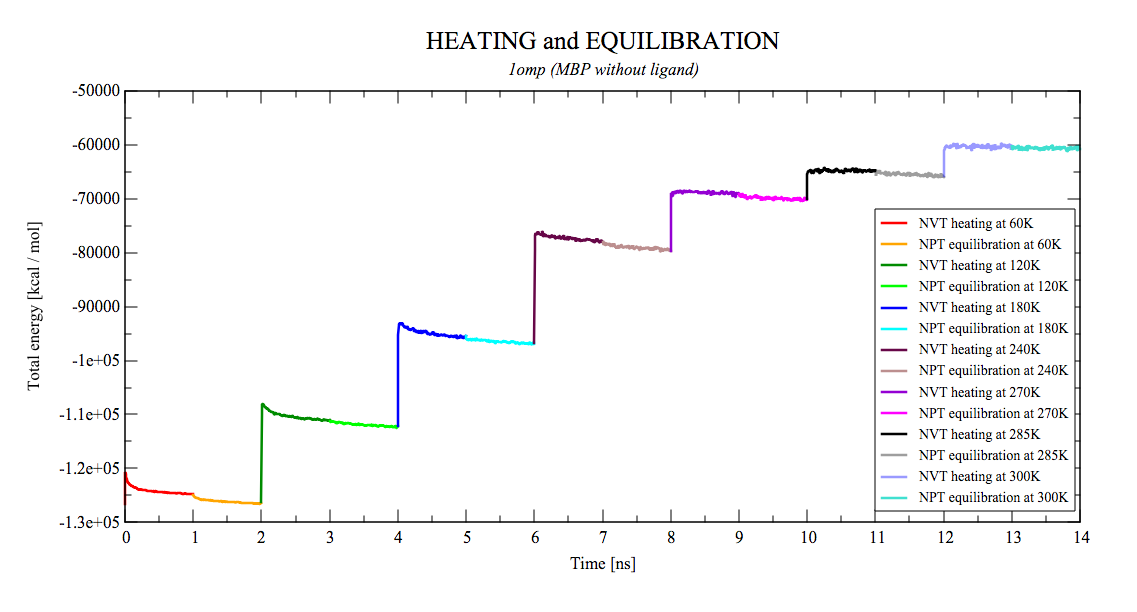
\includegraphics[width=\textwidth]{TOT-ht&eq.png}

\begin{figure}[H]
\centering
\begin{minipage}[t]{0.95\textwidth}
	\centering
    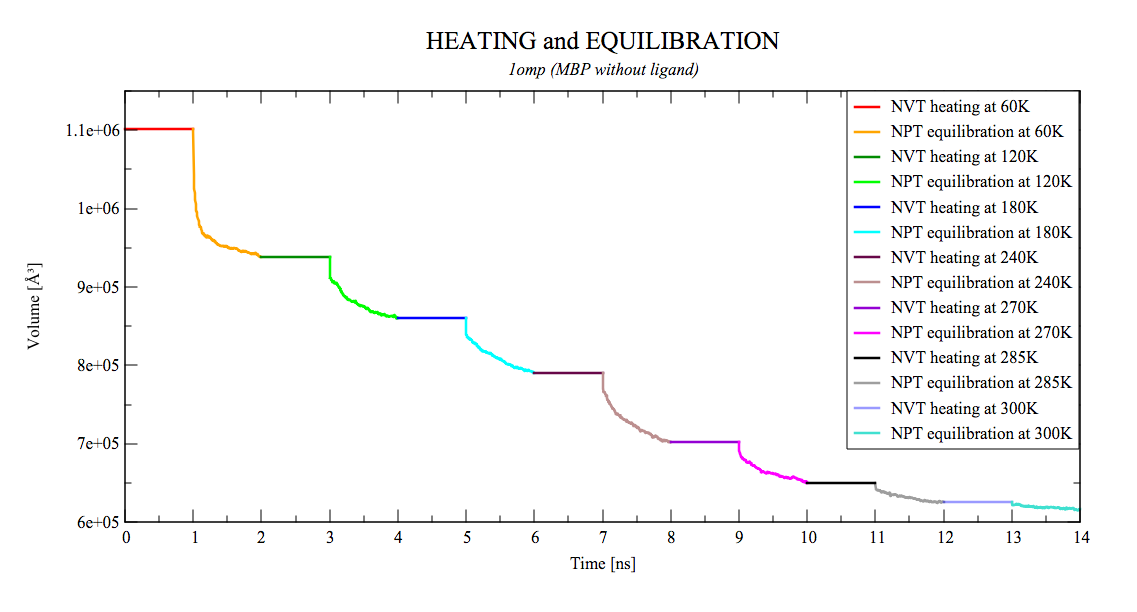
\includegraphics[width=\textwidth]{VOL-ht&eq.png}
    
    %\footnotesize{\caption{\textit{Graphs realized with QtGrace.}}
    %\label{fig:trj-trend}
    %}
\end{minipage} 
\end{figure}

\begin{figure}[H]
\centering
\begin{minipage}[t]{0.85\textwidth}
	\centering
    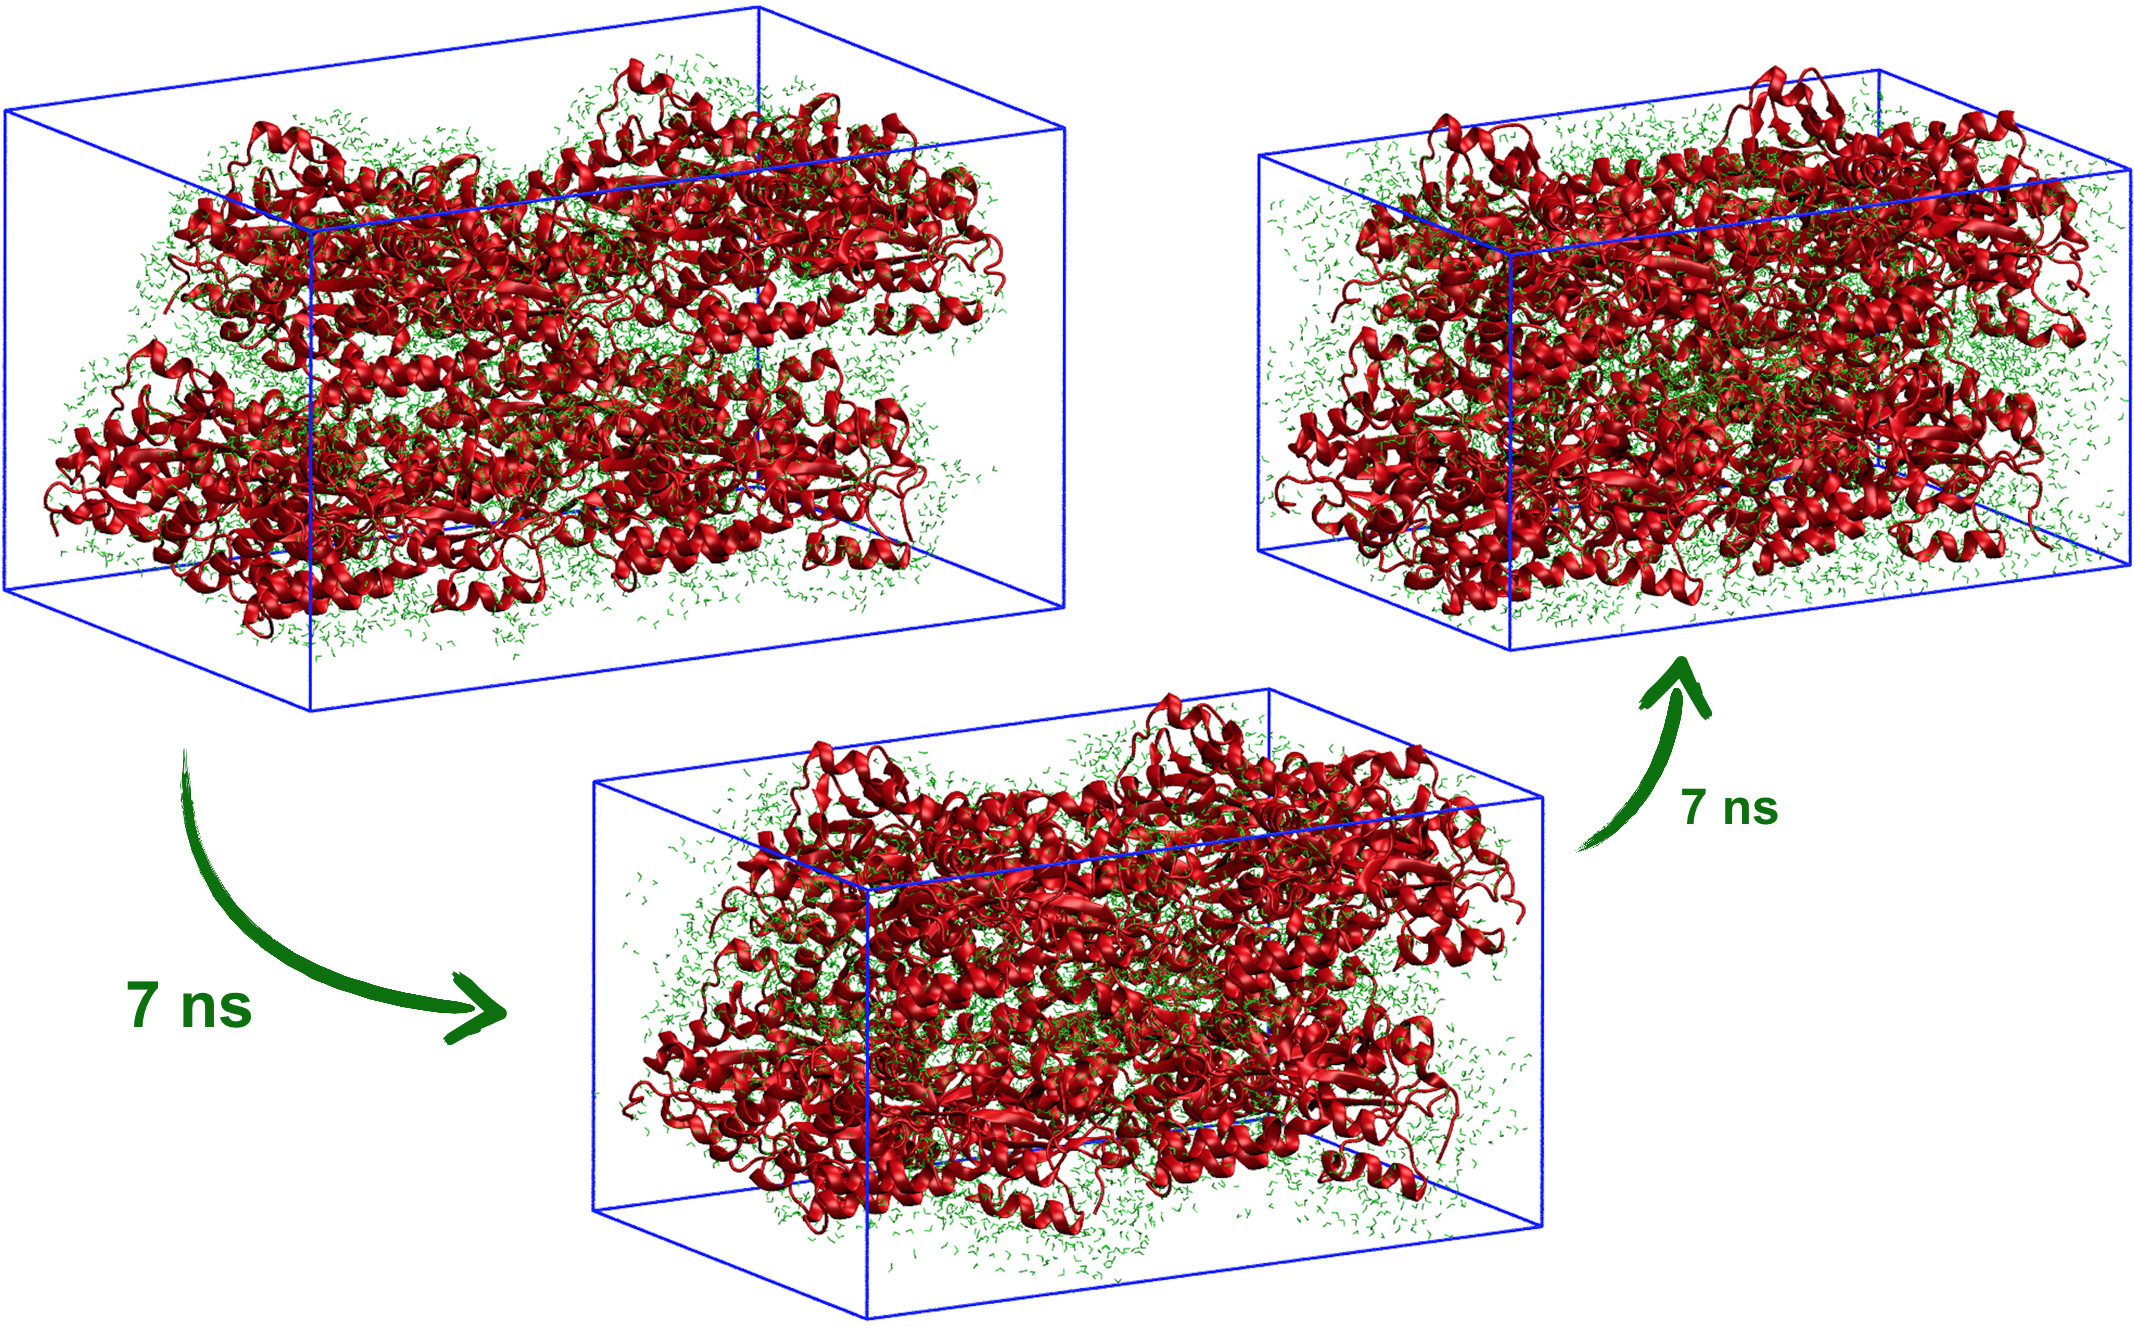
\includegraphics[width=0.9\textwidth]{h1.jpg}

\vspace{0.35cm}    
    
    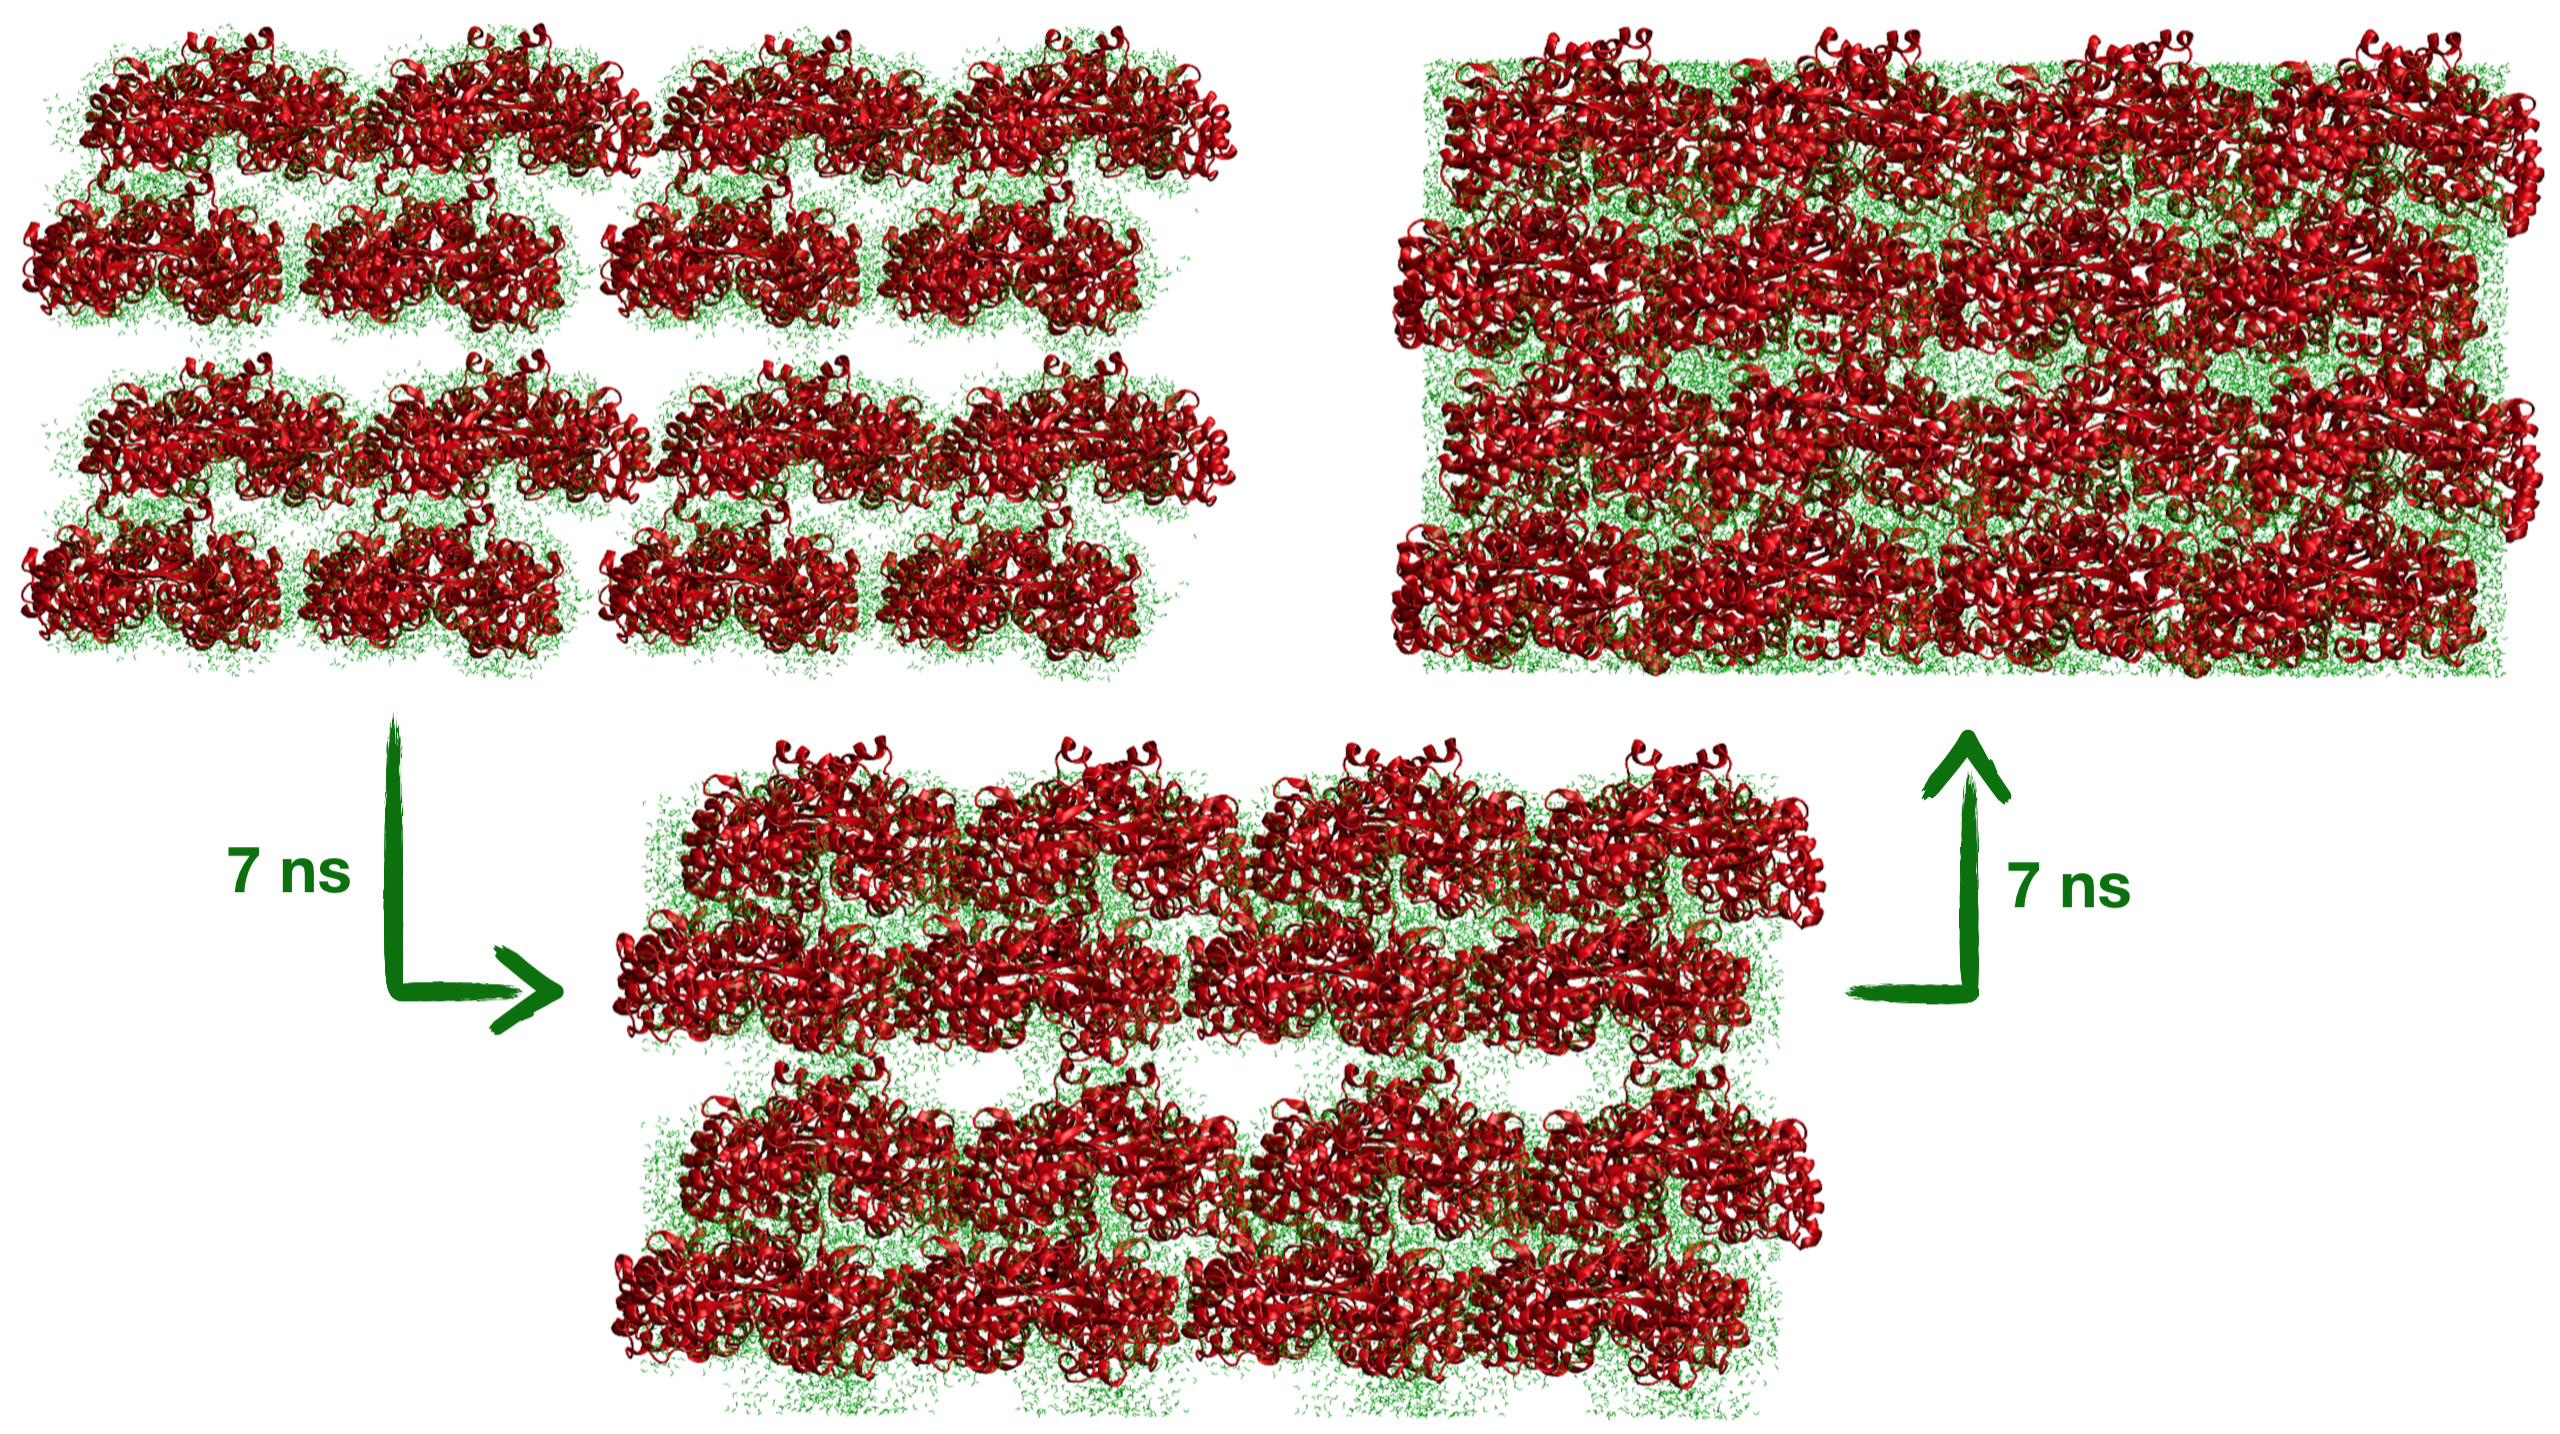
\includegraphics[width=0.9\textwidth]{h2.jpg}
    
    %\footnotesize{\caption{Heating and NPT equilibration. Results for the MBP system.}
    %\label{fig:trj-summ}
    %}
\end{minipage} 
\end{figure}

\item \textbf{Equilibration}\\
This is the last phase of the preparation of the starting state of the simulations. An NPT equilibration of 100 $ns$ at 300 K was carried out for each system. In order to achieve this, each simulation was divided into two runs of 50 $ns$. Moreover, it was evident that these systems were more stable in comparison to those manipulated in the previous phase, hence allowing to raise the \textit{timestep} from 1 $fs$ to 2 $fs$ and the \textit{PMEGridSpacing} from 1.3 to 2, and thus reducing the computational costs. In Fig. \ref{fig:trend-eq} the graphs on the evolution of the volume and the total energy of both systems are displayed.
%Questa è stata l'ultima fase della preparazione dello stato iniziale delle simulazioni. Si è eseguita una equilibratura di 100 $ns$ in NPT a 300 K su ciascun sistema. Per fare questo, ciascuna simulazione è stata divisa in due run da 50 $ns$ e, andando a svolgere delle simulazioni per tempi lunghi, si è tenuto conto che questi sistemi sono più stabili rispetto a quelli che erano stati trattati nella fase precedente permettendo così di aumentare sia il \textit{timestep}, da 1 $fs$ a 2 $fs$, che il \textit{PMEGridSpacing}, da 1.3 a 2, e ridurre così i costi computazionali. In Fig. \ref{} sono riportati i grafici dell'andamento del volume e dell'energia totale dei due sistemi nel corso dell'equilibratura.\\ 

\begin{figure}[H]
\centering
\begin{minipage}[t]{0.775\textwidth}
	\centering
    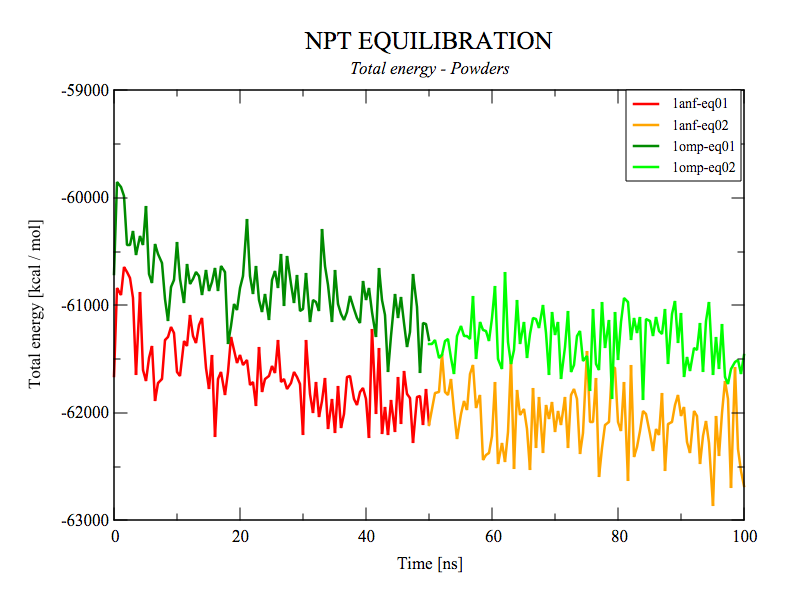
\includegraphics[width=0.9\textwidth]{total-energy.png}
    
    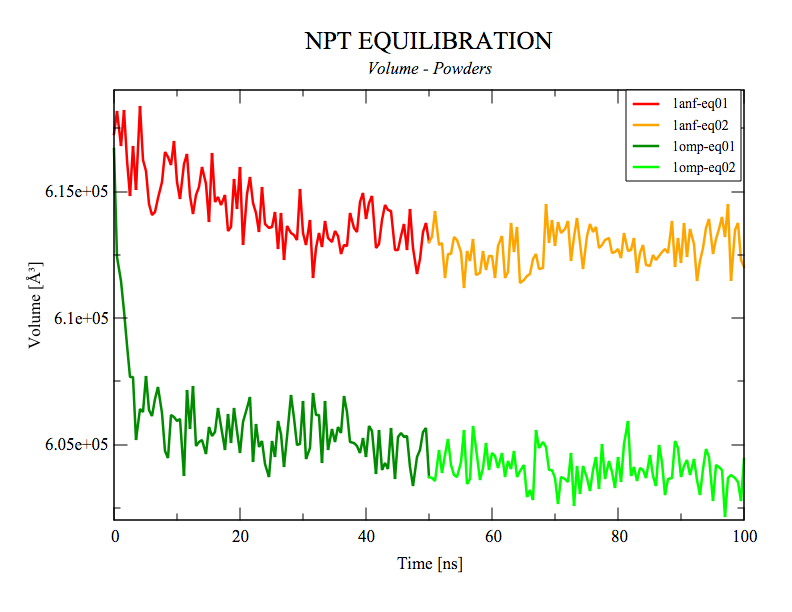
\includegraphics[width=0.9\textwidth]{volume.png}

    \footnotesize{\caption{Results of the energy minimization. \textit{Picture realized with QtGrace.}}
    \label{fig:trend-eq}
    }
\end{minipage} 
\end{figure}
\end{itemize}

\subsection{An appropriate water model}
Un altro importante risultato ottenuto da Tarek e Tobias riguarda the comparison between neutron-scattering experiments and water model used for the simulations.
In the analysis of their initial results obtained with the TIP3P model \cite{jorgensen1983comparison} for the H$_2$O molecules, they found poor agreement with the neutron data. Therefore, afterward they performed additional simulations with the SPC/E \cite{berendsen1987missing} model for the water molecules to investigate the dependence of the results on the water model. In this way, they discovered that the SPC/E model gives much better agreement than the TIP3P compared with neutron data.  
In particular this was clearly demonstrated by the density of states and the  the intermediate scattering functions, where both the modification of water dynamics from bulk behavior by the protein environment and its temperature dependence were accurately reproduced over a broad frequency range with the SPC/E model. The overall agreement with neutron data validates the methodologies and potential used, and provides a solid ground for accurately describing the water motion in relation to the protein dynamics and function  \cite{tarek2000dynamics}.

Quindi, puntando a realizzare delle simulazioni che possano essere utilizzare per analizzare più approfonditamente i dati emersi da recenti misure di neutron scattering, è bene tenere a questo risultato. Actually, nei file che descrivono il forcefield CHARMM (.top e .par), per le molecole d'acqua viene definito solo il modello TIP3P. Per facilitare la creazione degli stati iniziali dei due sistemi, si è deciso utilizzare inizialmente questo modello poiché is the CHARMM36 default model utilizzato per definire la forma e le interazioni delle molecole d'acqua. 

Realizzati gli stati iniziali si sono quindi andati a modificare i file (.psf) dei due sistemi e ad aggiungere i parametri del modello SPC/E nel file (.par) di CHARMM36. Dopo di che, per stabilizzare i sistemi, si è effettuata un'ulteriore equilibratura a 300 K di 50 $ns$.

\subsection{Production phase}
In questa fase, per studiare le simulazioni e trarre allo stesso tempo informazioni utili sui sistemi studiati, si è deciso di andare di andare ad eseguire due serie si simulazioni:
\begin{enumerate}
\item \textbf{Scan in temperature} per misurare la funzione di autorelazione temporale delle posizioni, ovvero i mean square displacement (MSD), degli atomi delle proteine nei diversi sistemi simulati in funzione della temperatura e della finestra temporale su cui viene colata la funzione di correlazione (nota anche come $t_w$ o \textit{time window}). Questo permette di studiare come cambiano le fluttuazioni medie degli atomi delle proteine per i diversi sistemi a diverse temperature. Hence, sono state eseguite several NPT simulations at different temperatures -- precisely: 200 K, 220 K, 240 K, 260 K, 280 K and 300K -- alternano fasi di equilibratura da 5 $ns$ con frequenza di campionamento\footnote{Per frequenza di campionamento si intende la frequenza con cui sono stati salvate le posizioni calcolate durante la simulazione. Una frequenza di campionamento di $(0.4 ps)^{-1}$ che la posizione viene salvata ogni 0.4 $ps$ e che quindi, per una simulazione di 5 $ns$ le traiettorie sono composte di 12,500 frames.} bassa $(1 ns)^{-1}$ e fasi di presa dati altrettanto lunghe dove la frequenza di campionamento è stata alzata a $(0.4 ps)^{-1}$. 
\item \textbf{Long time simulation} per andare ad approcciare una clustering analysis per studiare i cambiamenti conformazionali delle proteine. In questo caso, sono state fatte delle simulazioni di 1 $\mu s$ a 300 K. 
\end{enumerate}
In entrambi i casi, nei \textit{config} files delle diverse simulazioni performed for the production phase, i parametri del forcefield ed il PME sono stati impostati con i stessi setting used in the heating and equilibration phase della realizzazione dello stato iniziale.

\section{Results from the simulations}

